\documentclass{report}

%%%%%%%%%%%%%%%%%%%%%%%%%%%%%%%%%
% PACKAGE IMPORTS
%%%%%%%%%%%%%%%%%%%%%%%%%%%%%%%%%
\usepackage{titleps}
\usepackage[table]{xcolor}
\usepackage{tabularx}
\usepackage{multirow}
\usepackage{subfig}
\usepackage{bbding}
\usepackage{longtable}
\usepackage[tmargin=2cm,rmargin=1in,lmargin=1in,margin=0.85in,bmargin=2cm,footskip=.2in]{geometry}
\usepackage{amsmath,amsfonts,amsthm,amssymb,mathtools}
\usepackage[varbb]{newpxmath}
\usepackage{xfrac}
\usepackage[makeroom]{cancel}
\usepackage{mathtools}
\usepackage{bookmark}
\usepackage{enumitem}
\usepackage{hyperref,theoremref}
\hypersetup{
	pdftitle={Assignment},
	colorlinks=true, linkcolor=BrownPastel,
	bookmarksnumbered=true,
	bookmarksopen=true
}
\usepackage[most,many,breakable]{tcolorbox}
\usepackage{xcolor}
\usepackage{varwidth}
\usepackage{varwidth}
\usepackage{etoolbox}
%\usepackage{authblk}
\usepackage{nameref}
\usepackage{array}
\usepackage{multicol,array}
\usepackage{tikz-cd}
\usepackage[ruled,vlined,linesnumbered]{algorithm2e}
\usepackage{comment} % enables the use of multi-line comments (\ifx \fi) 
\usepackage{import}
\usepackage{xifthen}
\usepackage{pdfpages}
\usepackage{transparent}
\usepackage{afterpage}
\newcolumntype{C}[1]{>{\centering\arraybackslash}m{#1}}
\newcommand\mycommfont[1]{\footnotesize\ttfamily\textcolor{BrownPastel}{#1}}
\SetCommentSty{mycommfont}
\newcommand{\incfig}[1]{%
    \def\svgwidth{\columnwidth}
    \import{./figures/}{#1.pdf_tex}
}

\usepackage{tikzsymbols}
\renewcommand\qedsymbol{$\Laughey$}


%\usepackage{import}
%\usepackage{xifthen}
%\usepackage{pdfpages}
%\usepackage{transparent}


%%%%%%%%%%%%%%%%%%%%%%%%%%%%%%
% TEX LIVE PACKAGES
%%%%%%%%%%%%%%%%%%%%%%%%%%%%%%

\usepackage[T1]{fontenc}
\usepackage{anyfontsize}

%%%%%%%%%%%%%%%%%%%%%%%%%%%%%%
% BLANK PAGE
%%%%%%%%%%%%%%%%%%%%%%%%%%%%%%

\newcommand\blankpage{%
    \null
    \thispagestyle{empty}%
    \newpage
}

%%%%%%%%%%%%%%%%%%%%%%%%%%%%%%
% SOME COOL COLORS
%%%%%%%%%%%%%%%%%%%%%%%%%%%%%%

\definecolor{RedPastel}{RGB}{255, 204, 204}
\definecolor{OrangePastel}{RGB}{255, 224, 204}
\definecolor{BrownPastel}{RGB}{229, 204, 170}
\definecolor{GreenPastel}{RGB}{204, 255, 204}
\definecolor{BluePastel}{RGB}{204, 229, 255}
\definecolor{PurplePastel}{RGB}{229, 204, 255}

\newcommand{\evidence}[1]{%
    \textcolor{cyan}{\textit{#1}}%
}

\newcommand{\glitter}[1]{%
    \textcolor{green}{\textit{#1}}%
}

\newcommand{\fancyglitter}[1]{%
    \textcolor{red}{\textit{#1}}%
}

\newcommand{\newfancyglitter}[1]{%
    \textcolor{violet}{\textit{#1}}%
}

%%%%%%%%%%%%%%%%%%%%%%%%%%%%%%
% SELF MADE COLORS
%%%%%%%%%%%%%%%%%%%%%%%%%%%%%%



\definecolor{myg}{RGB}{56, 140, 70}
\definecolor{myb}{RGB}{45, 111, 177}
\definecolor{myr}{RGB}{199, 68, 64}
\definecolor{mytheorembg}{HTML}{F2F2F9}
\definecolor{mytheoremfr}{HTML}{00007B}
\definecolor{mylenmabg}{HTML}{FFFAF8}
\definecolor{mylenmafr}{HTML}{983b0f}
\definecolor{mypropbg}{HTML}{f2fbfc}
\definecolor{mypropfr}{HTML}{191971}
\definecolor{myexamplebg}{HTML}{F2FBF8}
\definecolor{myexamplefr}{HTML}{88D6D1}
\definecolor{myexampleti}{HTML}{2A7F7F}
\definecolor{mydefinitbg}{HTML}{E5E5FF}
\definecolor{mydefinitfr}{HTML}{3F3FA3}
\definecolor{notesred}{RGB}{0,162,0}
\definecolor{myp}{RGB}{197, 92, 212}
\definecolor{mygr}{HTML}{2C3338}
\definecolor{BrownPasteled}{RGB}{127,0,0}
\definecolor{myyellow}{RGB}{169,121,69}
\definecolor{myexercisebg}{HTML}{F2FBF8}
\definecolor{myexercisefg}{HTML}{88D6D1}


%%%%%%%%%%%%%%%%%%%%%%%%%%%%
% TCOLORBOX SETUPS
%%%%%%%%%%%%%%%%%%%%%%%%%%%%

\setlength{\parindent}{1cm}
%================================
% THEOREM BOX
%================================

\tcbuselibrary{theorems,skins,hooks}
\newtcbtheorem[number within=section]{Theorem}{Teorema}
{%
	enhanced,
	breakable,
	colback = mytheorembg,
	frame hidden,
	boxrule = 0sp,
	borderline west = {2pt}{0pt}{mytheoremfr},
	sharp corners,
	detach title,
	before upper = \tcbtitle\par\smallskip,
	coltitle = mytheoremfr,
	fonttitle = \bfseries\sffamily,
	description font = \mdseries,
	separator sign none,
	segmentation style={solid, mytheoremfr},
}
{th}

\tcbuselibrary{theorems,skins,hooks}
\newtcbtheorem[number within=chapter]{theorem}{Theorem}
{%
	enhanced,
	breakable,
	colback = mytheorembg,
	frame hidden,
	boxrule = 0sp,
	borderline west = {2pt}{0pt}{mytheoremfr},
	sharp corners,
	detach title,
	before upper = \tcbtitle\par\smallskip,
	coltitle = mytheoremfr,
	fonttitle = \bfseries\sffamily,
	description font = \mdseries,
	separator sign none,
	segmentation style={solid, mytheoremfr},
}
{th}


\tcbuselibrary{theorems,skins,hooks}
\newtcolorbox{Theoremcon}
{%
	enhanced
	,breakable
	,colback = mytheorembg
	,frame hidden
	,boxrule = 0sp
	,borderline west = {2pt}{0pt}{mytheoremfr}
	,sharp corners
	,description font = \mdseries
	,separator sign none
}

%================================
% Corollery
%================================
\tcbuselibrary{theorems,skins,hooks}
\newtcbtheorem[number within=section]{Corollary}{Corollario}
{%
	enhanced
	,breakable
	,colback = myp!10
	,frame hidden
	,boxrule = 0sp
	,borderline west = {2pt}{0pt}{myp!85!black}
	,sharp corners
	,detach title
	,before upper = \tcbtitle\par\smallskip
	,coltitle = myp!85!black
	,fonttitle = \bfseries\sffamily
	,description font = \mdseries
	,separator sign none
	,segmentation style={solid, myp!85!black}
}
{th}
\tcbuselibrary{theorems,skins,hooks}
\newtcbtheorem[number within=chapter]{corollary}{Corollary}
{%
	enhanced
	,breakable
	,colback = myp!10
	,frame hidden
	,boxrule = 0sp
	,borderline west = {2pt}{0pt}{myp!85!black}
	,sharp corners
	,detach title
	,before upper = \tcbtitle\par\smallskip
	,coltitle = myp!85!black
	,fonttitle = \bfseries\sffamily
	,description font = \mdseries
	,separator sign none
	,segmentation style={solid, myp!85!black}
}
{th}


%================================
% LENMA
%================================

\tcbuselibrary{theorems,skins,hooks}
\newtcbtheorem{Lenma}{Eserczio}
{%
	enhanced,
	breakable,
	colback = mylenmabg,
	frame hidden,
	boxrule = 0sp,
	borderline west = {2pt}{0pt}{mylenmafr},
	sharp corners,
	detach title,
	before upper = \tcbtitle\par\smallskip,
	coltitle = mylenmafr,
	fonttitle = \bfseries\sffamily,
	description font = \mdseries,
	separator sign none,
	segmentation style={solid, mylenmafr},
}
{th}

\tcbuselibrary{theorems,skins,hooks}
\newtcbtheorem[number within=chapter]{lenma}{Lenma}
{%
	enhanced,
	breakable,
	colback = mylenmabg,
	frame hidden,
	boxrule = 0sp,
	borderline west = {2pt}{0pt}{mylenmafr},
	sharp corners,
	detach title,
	before upper = \tcbtitle\par\smallskip,
	coltitle = mylenmafr,
	fonttitle = \bfseries\sffamily,
	description font = \mdseries,
	separator sign none,
	segmentation style={solid, mylenmafr},
}
{th}


%================================
% PROPOSITION
%================================

\tcbuselibrary{theorems,skins,hooks}
\newtcbtheorem[number within=section]{Prop}{Proposition}
{%
	enhanced,
	breakable,
	colback = mypropbg,
	frame hidden,
	boxrule = 0sp,
	borderline west = {2pt}{0pt}{mypropfr},
	sharp corners,
	detach title,
	before upper = \tcbtitle\par\smallskip,
	coltitle = mypropfr,
	fonttitle = \bfseries\sffamily,
	description font = \mdseries,
	separator sign none,
	segmentation style={solid, mypropfr},
}
{th}

\tcbuselibrary{theorems,skins,hooks}
\newtcbtheorem[number within=chapter]{prop}{Proposition}
{%
	enhanced,
	breakable,
	colback = mypropbg,
	frame hidden,
	boxrule = 0sp,
	borderline west = {2pt}{0pt}{mypropfr},
	sharp corners,
	detach title,
	before upper = \tcbtitle\par\smallskip,
	coltitle = mypropfr,
	fonttitle = \bfseries\sffamily,
	description font = \mdseries,
	separator sign none,
	segmentation style={solid, mypropfr},
}
{th}
%================================
% PATTERN
%================================

\usepackage[most]{tcolorbox}

\definecolor{mypatternbg}{RGB}{255,248,220} 
\definecolor{mypatternfr}{RGB}{139,69,19} 

\tcbuselibrary{theorems,skins,hooks}

\newtcbtheorem[number within=section]{Pattern}{Pattern}
{%
    enhanced,
    breakable,
    colback = mypatternbg,
    boxrule = 0.75mm,
    colframe = mypatternfr,
    colbacktitle = mypatternfr!20,
    coltitle = black,
    fonttitle = \bfseries,
    sharp corners,
    detach title,
    before upper = \tcbtitle\par\smallskip,
    description font = \mdseries\itshape,
    separator sign none,
    segmentation style={solid, mypatternfr},
    theorem style=plain,
}
{th}

%================================
% OBSERVATION
%================================

\definecolor{myg}{RGB}{0,128,0} % Define your color myg

\tcbuselibrary{theorems,skins,hooks}
\definecolor{mytheorembg}{RGB}{255,248,220}
\definecolor{mytheoremfr}{RGB}{139,69,19}
\definecolor{myb}{RGB}{0,0,255}

\tcbuselibrary{theorems,skins,hooks}

\newtcbtheorem[number within=section]{Observation}{Osservazione}
{%
    enhanced,
    breakable,
    colback = mytheorembg,
    frame hidden,
    boxrule = 0sp,
    borderline west = {2pt}{0pt}{mytheoremfr},
    sharp corners,
    detach title,
    before upper = \tcbtitle\par\smallskip,
    coltitle = mytheoremfr,
    fonttitle = \bfseries\sffamily,
    description font = \mdseries,
    separator sign none,
    segmentation style={solid, mytheoremfr},
    attach boxed title to top left={yshift*=-\tcboxedtitleheight},
    fonttitle=\bfseries,
    boxed title size=title,
    boxed title style={%
        sharp corners,
        rounded corners=northwest,
        colback=myb!80!black,
        boxrule=0pt,
    },
    underlay boxed title={%
        \path[fill=myb!80!black] (title.south west)--(title.south east)
        to[out=0, in=180] ([xshift=5mm]title.east)--
        (title.center-|frame.east)
        [rounded corners=\kvtcb@arc] |-
        (frame.north) -| cycle;
    },
}
{th}
%================================
% CLAIM
%================================

\tcbuselibrary{theorems,skins,hooks}
\newtcbtheorem[number within=section]{claim}{Osservazioni}
{%
	enhanced
	,breakable
	,colback = myg!10
	,frame hidden
	,boxrule = 0sp
	,borderline west = {2pt}{0pt}{myg}
	,sharp corners
	,detach title
	,before upper = \tcbtitle\par\smallskip
	,coltitle = myg!85!black
	,fonttitle = \bfseries\sffamily
	,description font = \mdseries
	,separator sign none
	,segmentation style={solid, myg!85!black}
}
{th}



%================================
% Exercise
%================================

\tcbuselibrary{theorems,skins,hooks}
\newtcbtheorem[number within=section]{Exercise}{Problema}
{%
	enhanced,
	breakable,
	colback = myexercisebg,
	frame hidden,
	boxrule = 0sp,
	borderline west = {2pt}{0pt}{myexercisefg},
	sharp corners,
	detach title,
	before upper = \tcbtitle\par\smallskip,
	coltitle = myexercisefg,
	fonttitle = \bfseries\sffamily,
	description font = \mdseries,
	separator sign none,
	segmentation style={solid, myexercisefg},
}
{th}

\tcbuselibrary{theorems,skins,hooks}
\newtcbtheorem[number within=chapter]{exercise}{Exercise}
{%
	enhanced,
	breakable,
	colback = myexercisebg,
	frame hidden,
	boxrule = 0sp,
	borderline west = {2pt}{0pt}{myexercisefg},
	sharp corners,
	detach title,
	before upper = \tcbtitle\par\smallskip,
	coltitle = myexercisefg,
	fonttitle = \bfseries\sffamily,
	description font = \mdseries,
	separator sign none,
	segmentation style={solid, myexercisefg},
}
{th}

%================================
% EXAMPLE BOX
%================================

\newtcbtheorem[number within=section]{Example}{Esempio}
{%
	colback = myexamplebg
	,breakable
	,colframe = myexamplefr
	,coltitle = myexampleti
	,boxrule = 1pt
	,sharp corners
	,detach title
	,before upper=\tcbtitle\par\smallskip
	,fonttitle = \bfseries
	,description font = \mdseries
	,separator sign none
	,description delimiters parenthesis
}
{ex}

\newtcbtheorem[number within=chapter]{example}{Esempio}
{%
	colback = myexamplebg
	,breakable
	,colframe = myexamplefr
	,coltitle = myexampleti
	,boxrule = 1pt
	,sharp corners
	,detach title
	,before upper=\tcbtitle\par\smallskip
	,fonttitle = \bfseries
	,description font = \mdseries
	,separator sign none
	,description delimiters parenthesis
}
{ex}

%================================
% DEFINITION BOX
%================================

\newtcbtheorem[number within=section]{Definizione}{Definizione}{enhanced,
	before skip=2mm,after skip=2mm, colback=red!5,colframe=red!80!black,boxrule=0.5mm,
	attach boxed title to top left={xshift=1cm,yshift*=1mm-\tcboxedtitleheight}, varwidth boxed title*=-3cm,
	boxed title style={frame code={
					\path[fill=tcbcolback]
					([yshift=-1mm,xshift=-1mm]frame.north west)
					arc[start angle=0,end angle=180,radius=1mm]
					([yshift=-1mm,xshift=1mm]frame.north east)
					arc[start angle=180,end angle=0,radius=1mm];
					\path[left color=tcbcolback!60!black,right color=tcbcolback!60!black,
						middle color=tcbcolback!80!black]
					([xshift=-2mm]frame.north west) -- ([xshift=2mm]frame.north east)
					[rounded corners=1mm]-- ([xshift=1mm,yshift=-1mm]frame.north east)
					-- (frame.south east) -- (frame.south west)
					-- ([xshift=-1mm,yshift=-1mm]frame.north west)
					[sharp corners]-- cycle;
				},interior engine=empty,
		},
	fonttitle=\bfseries,
	title={#2},#1}{def}
\newtcbtheorem[number within=chapter]{definizione}{Definizione}{enhanced,
	before skip=2mm,after skip=2mm, colback=red!5,colframe=red!80!black,boxrule=0.5mm,
	attach boxed title to top left={xshift=1cm,yshift*=1mm-\tcboxedtitleheight}, varwidth boxed title*=-3cm,
	boxed title style={frame code={
					\path[fill=tcbcolback]
					([yshift=-1mm,xshift=-1mm]frame.north west)
					arc[start angle=0,end angle=180,radius=1mm]
					([yshift=-1mm,xshift=1mm]frame.north east)
					arc[start angle=180,end angle=0,radius=1mm];
					\path[left color=tcbcolback!60!black,right color=tcbcolback!60!black,
						middle color=tcbcolback!80!black]
					([xshift=-2mm]frame.north west) -- ([xshift=2mm]frame.north east)
					[rounded corners=1mm]-- ([xshift=1mm,yshift=-1mm]frame.north east)
					-- (frame.south east) -- (frame.south west)
					-- ([xshift=-1mm,yshift=-1mm]frame.north west)
					[sharp corners]-- cycle;
				},interior engine=empty,
		},
	fonttitle=\bfseries,
	title={#2},#1}{def}



%================================
% Solution BOX
%================================

\makeatletter
\newtcbtheorem[number within=chapter]{question}{Domanda}{enhanced,
	breakable,
	colback=white,
	colframe=myb!80!black,
	attach boxed title to top left={yshift*=-\tcboxedtitleheight},
	fonttitle=\bfseries,
	title={#2},
	boxed title size=title,
	boxed title style={%
			sharp corners,
			rounded corners=northwest,
			colback=tcbcolframe,
			boxrule=0pt,
		},
	underlay boxed title={%
			\path[fill=tcbcolframe] (title.south west)--(title.south east)
			to[out=0, in=180] ([xshift=5mm]title.east)--
			(title.center-|frame.east)
			[rounded corners=\kvtcb@arc] |-
			(frame.north) -| cycle;
		},
	#1
}{def}
\makeatother

%================================
% SOLUTION BOX
%================================

\makeatletter
\newtcolorbox{solution}{enhanced,
	breakable,
	colback=white,
	colframe=myg!80!black,
	attach boxed title to top left={yshift*=-\tcboxedtitleheight},
	title=Risposta,
	boxed title size=title,
	boxed title style={%
			sharp corners,
			rounded corners=northwest,
			colback=tcbcolframe,
			boxrule=0pt,
		},
	underlay boxed title={%
			\path[fill=tcbcolframe] (title.south west)--(title.south east)
			to[out=0, in=180] ([xshift=5mm]title.east)--
			(title.center-|frame.east)
			[rounded corners=\kvtcb@arc] |-
			(frame.north) -| cycle;
		},
}
\makeatother

%================================
% Question BOX
%================================

\makeatletter
\newtcbtheorem{qstion}{Question}{enhanced,
	breakable,
	colback=white,
	colframe=mygr,
	attach boxed title to top left={yshift*=-\tcboxedtitleheight},
	fonttitle=\bfseries,
	title={#2},
	boxed title size=title,
	boxed title style={%
			sharp corners,
			rounded corners=northwest,
			colback=tcbcolframe,
			boxrule=0pt,
		},
	underlay boxed title={%
			\path[fill=tcbcolframe] (title.south west)--(title.south east)
			to[out=0, in=180] ([xshift=5mm]title.east)--
			(title.center-|frame.east)
			[rounded corners=\kvtcb@arc] |-
			(frame.north) -| cycle;
		},
	#1
}{def}
\makeatother

\newtcbtheorem[number within=chapter]{wconc}{Concetto sbagliato}{
	breakable,
	enhanced,
	colback=white,
	colframe=myr,
	arc=0pt,
	outer arc=0pt,
	fonttitle=\bfseries\sffamily\large,
	colbacktitle=myr,
	attach boxed title to top left={},
	boxed title style={
			enhanced,
			skin=enhancedfirst jigsaw,
			arc=3pt,
			bottom=0pt,
			interior style={fill=myr}
		},
	#1
}{def}


%================================
% CODE BOX
%================================

\usetikzlibrary{arrows,calc,shadows.blur}
\tcbuselibrary{skins}
\newtcolorbox{code}[1][]{%
	enhanced jigsaw,
	colback=pink,%
	colframe=pink,
	size=small,
	before skip=2mm, after skip=2mm,
	boxrule=1pt,
	title=\textbf{Struttura del Pattern},
	halign title=flush center,
	coltitle=black,
	breakable,
	drop shadow=black!50!white,
	attach boxed title to top center = {yshift=-\tcboxedtitleheight/2},
	minipage boxed title=5cm,
	boxed title style={%
			colback=OrangePastel,
			size=fbox,
			boxrule=1pt,
			boxsep=2pt,
			underlay={%
					\coordinate (dotA) at ($(interior.west) + (-0.5pt,0)$);
					\coordinate (dotB) at ($(interior.east) + (0.5pt,0)$);
					\begin{scope}
						\clip (interior.north west) rectangle ([xshift=3ex]interior.east);
						\filldraw [OrangePastel, blur shadow={shadow opacity=60, shadow yshift=-.75ex}, rounded corners=2pt] (interior.north west) rectangle (interior.south east);
					\end{scope}
					\begin{scope}[gray!80!black]
						\fill (dotA) circle (2pt);
						\fill (dotB) circle (2pt);
					\end{scope}
				},
		},
	#1,
}

%================================
% NOTE BOX
%================================

\usetikzlibrary{arrows,calc,shadows.blur}
\tcbuselibrary{skins}
\newtcolorbox{note}[1][]{%
	enhanced jigsaw,
	colback=gray!20!white,%
	colframe=gray!80!black,
	size=small,
	boxrule=1pt,
	title=\textbf{Note:-},
	halign title=flush center,
	coltitle=black,
	breakable,
	drop shadow=black!50!white,
	attach boxed title to top left={xshift=1cm,yshift=-\tcboxedtitleheight/2,yshifttext=-\tcboxedtitleheight/2},
	minipage boxed title=1.5cm,
	boxed title style={%
			colback=white,
			size=fbox,
			boxrule=1pt,
			boxsep=2pt,
			underlay={%
					\coordinate (dotA) at ($(interior.west) + (-0.5pt,0)$);
					\coordinate (dotB) at ($(interior.east) + (0.5pt,0)$);
					\begin{scope}
						\clip (interior.north west) rectangle ([xshift=3ex]interior.east);
						\filldraw [white, blur shadow={shadow opacity=60, shadow yshift=-.75ex}, rounded corners=2pt] (interior.north west) rectangle (interior.south east);
					\end{scope}
					\begin{scope}[gray!80!black]
						\fill (dotA) circle (2pt);
						\fill (dotB) circle (2pt);
					\end{scope}
				},
		},
	#1,
}

%%%%%%%%%%%%%%%%%%%%%%%%%%%%%%
% SELF MADE COMMANDS
%%%%%%%%%%%%%%%%%%%%%%%%%%%%%%


\newcommand{\thm}[2]{\begin{Theorem}{#1}{}#2\end{Theorem}}
\newcommand{\cor}[2]{\begin{Corollary}{#1}{}#2\end{Corollary}}
\newcommand{\mlenma}[2]{\begin{Lenma}{#1}{}#2\end{Lenma}}
\newcommand{\mprop}[2]{\begin{Prop}{#1}{}#2\end{Prop}}
\newcommand{\clm}[3]{\begin{claim}{#1}{#2}#3\end{claim}}
\newcommand{\wc}[2]{\begin{wconc}{#1}{}#2\end{wconc}}
\newcommand{\thmcon}[1]{\begin{Theoremcon}{#1}\end{Theoremcon}}
\newcommand{\ex}[2]{\begin{Example}{#1}{}#2\end{Example}}
\newcommand{\dfn}[2]{\begin{Definizione}[colbacktitle=red!75!black]{#1}{}#2\end{Definizione}}
\newcommand{\dfnc}[2]{\begin{definizione}[colbacktitle=red!75!black]{#1}{}#2\end{definizione}}
\newcommand{\qs}[2]{\begin{question}{#1}{}#2\end{question}}
\newcommand{\pf}[2]{\begin{myproof}[#1]#2\end{myproof}}
\newcommand{\nt}[1]{\begin{note}#1\end{note}}
\newcommand{\cd}[1]{\begin{code}#1\end{code}}
\newcommand{\mypattern}[2]{\begin{Pattern}{#1}{}#2\end{Pattern}}
\newcommand{\obs}[2]{\begin{Observation}{#1}{}#2\end{Observation}}

\newcommand*\circled[1]{\tikz[baseline=(char.base)]{
		\node[shape=circle,draw,inner sep=1pt] (char) {#1};}}
\newcommand\getcurrentref[1]{%
	\ifnumequal{\value{#1}}{0}
	{??}
	{\the\value{#1}}%
}
\newcommand{\getCurrentSectionNumber}{\getcurrentref{section}}
\newenvironment{myproof}[1][\proofname]{%
	\proof[\bfseries #1: ]%
}{\endproof}

\newcommand{\mclm}[2]{\begin{myclaim}[#1]#2\end{myclaim}}
\newenvironment{myclaim}[1][\claimname]{\proof[\bfseries #1: ]}{}

\newcounter{mylabelcounter}

\makeatletter
\newcommand{\setword}[2]{%
	\phantomsection
	#1\def\@currentlabel{\unexpanded{#1}}\label{#2}%
}
\makeatother




\tikzset{
	symbol/.style={
			draw=none,
			every to/.append style={
					edge node={node [sloped, allow upside down, auto=false]{$#1$}}}
		}
}


% deliminators
\DeclarePairedDelimiter{\abs}{\lvert}{\rvert}
\DeclarePairedDelimiter{\norm}{\lVert}{\rVert}

\DeclarePairedDelimiter{\ceil}{\lceil}{\rceil}
\DeclarePairedDelimiter{\floor}{\lfloor}{\rfloor}
\DeclarePairedDelimiter{\round}{\lfloor}{\rceil}

\newsavebox\diffdbox
\newcommand{\slantedromand}{{\mathpalette\makesl{d}}}
\newcommand{\makesl}[2]{%
\begingroup
\sbox{\diffdbox}{$\mathsurround=0pt#1\mathrm{#2}$}%
\pdfsave
\pdfsetmatrix{1 0 0.2 1}%
\rlap{\usebox{\diffdbox}}%
\pdfrestore
\hskip\wd\diffdbox
\endgroup
}
\newcommand{\dd}[1][]{\ensuremath{\mathop{}\!\ifstrempty{#1}{%
\slantedromand\@ifnextchar^{\hspace{0.2ex}}{\hspace{0.1ex}}}%
{\slantedromand\hspace{0.2ex}^{#1}}}}
\ProvideDocumentCommand\dv{o m g}{%
  \ensuremath{%
    \IfValueTF{#3}{%
      \IfNoValueTF{#1}{%
        \frac{\dd #2}{\dd #3}%
      }{%
        \frac{\dd^{#1} #2}{\dd #3^{#1}}%
      }%
    }{%
      \IfNoValueTF{#1}{%
        \frac{\dd}{\dd #2}%
      }{%
        \frac{\dd^{#1}}{\dd #2^{#1}}%
      }%
    }%
  }%
}
\providecommand*{\pdv}[3][]{\frac{\partial^{#1}#2}{\partial#3^{#1}}}
%  - others
\DeclareMathOperator{\Lap}{\mathcal{L}}
\DeclareMathOperator{\Var}{Var} % varience
\DeclareMathOperator{\Cov}{Cov} % covarience
\DeclareMathOperator{\E}{E} % expected

% Since the amsthm package isn't loaded

% I prefer the slanted \leq
\let\oldleq\leq % save them in case they're every wanted
\let\oldgeq\geq
\renewcommand{\leq}{\leqslant}
\renewcommand{\geq}{\geqslant}

% % redefine matrix env to allow for alignment, use r as default
% \renewcommand*\env@matrix[1][r]{\hskip -\arraycolsep
%     \let\@ifnextchar\new@ifnextchar
%     \array{*\c@MaxMatrixCols #1}}


%\usepackage{framed}
%\usepackage{titletoc}
%\usepackage{etoolbox}
%\usepackage{lmodern}


%\patchcmd{\tableofcontents}{\contentsname}{\sffamily\contentsname}{}{}

%\renewenvironment{leftbar}
%{\def\FrameCommand{\hspace{6em}%
%		{\color{myyellow}\vrule width 2pt depth 6pt}\hspace{1em}}%
%	\MakeFramed{\parshape 1 0cm \dimexpr\textwidth-6em\relax\FrameRestore}\vskip2pt%
%}
%{\endMakeFramed}

%\titlecontents{chapter}
%[0em]{\vspace*{2\baselineskip}}
%{\parbox{4.5em}{%
%		\hfill\Huge\sffamily\bfseries\color{BrownPasteled}\thecontentspage}%
%	\vspace*{-2.3\baselineskip}\leftbar\textsc{\small\chaptername~\thecontentslabel}\\\sffamily}
%{}{\endleftbar}
%\titlecontents{section}
%[8.4em]
%{\sffamily\contentslabel{3em}}{}{}
%{\hspace{0.5em}\nobreak\itshape\color{BrownPasteled}\contentspage}
%\titlecontents{subsection}
%[8.4em]
%{\sffamily\contentslabel{3em}}{}{}  
%{\hspace{0.5em}\nobreak\itshape\color{BrownPasteled}\contentspage}



%%%%%%%%%%%%%%%%%%%%%%%%%%%%%%%%%%%%%%%%%%%
% TABLE OF CONTENTS
%%%%%%%%%%%%%%%%%%%%%%%%%%%%%%%%%%%%%%%%%%%

\definecolor{1}{rgb}{0.7,0,0}
\definecolor{2}{rgb}{0,0.7,0}
\definecolor{3}{rgb}{0,0,0.7}
\definecolor{4}{rgb}{1,0.75,0}
\definecolor{5}{rgb}{1,0.75,0.8}
\definecolor{6}{rgb}{0,0.13, 0.38}
\definecolor{7}{rgb}{0.21,0.37,0.23}
\definecolor{8}{rgb}{0.5,0.5,0.5}

\newcommand{\ChapterColor}[1]{%
    \ifcase#1\relax
    \or \color{1}%
    \or \color{2}%
    \or \color{3}%
	\or \color{4}%
	\or \color{5}%
	\or \color{6}%
	\or \color{7}%
	\or \color{8}%
    \else \color{black}%
    \fi
}

\newcommand{\chapterColor}[1]{%
    \ifcase#1\relax
    \or 1%
    \or 2%
    \or 3%
	\or 4%
	\or 5%
	\or 6%
	\or 7%
	\or 8%
    \else black%
    \fi
}

\usepackage{tikz}
\definecolor{doc}{RGB}{0,60,110}
\usepackage{titletoc}
\contentsmargin{0cm}
\titlecontents{chapter}[3.7pc]
{\addvspace{30pt}%
	\begin{tikzpicture}[remember picture, overlay]%
		\draw[fill=\chapterColor{\thecontentslabel},draw=\chapterColor{\thecontentslabel}] (-7.3,-.1) rectangle (-0.5,.5);%
		\pgftext[left,x=-3.7cm,y=0.2cm]{\color{white}\Large\sc\bfseries Capitolo\ \thecontentslabel};%
	\end{tikzpicture}\ChapterColor{\thecontentslabel}\large\sc\bfseries}%
{}
{}
{\;\titlerule\;\ChapterColor{\thecontentslabel}\large\sc\bfseries Pagina \thecontentspage
	\begin{tikzpicture}[remember picture, overlay]
		\draw[fill=,draw=\chapterColor{\thecontentslabel}] (2pt,0) rectangle (4,0.1pt);
	\end{tikzpicture}}%
\titlecontents{section}[3.7pc]
{\addvspace{2pt}}
{\contentslabel[\thecontentslabel]{2pc}}
{}
{\hfill\small \thecontentspage}
[]
\titlecontents*{subsection}[3.7pc]
{\addvspace{-1pt}\small}
{}
{}
{\ --- \small\thecontentspage}
[ \textbullet\ ][]

\makeatletter
\renewcommand{\chaptername}{Capitolo}
\renewcommand{\tableofcontents}{%
	\chapter*{%
	  \vspace*{-20\p@}%
	  \begin{tikzpicture}[remember picture, overlay]%
		  \pgftext[right,x=15cm,y=0.2cm]{\color{BrownPastel}\Huge\sc\bfseries \contentsname};%
		  \draw[fill=BrownPastel,draw=BrownPastel] (13,-.75) rectangle (20,1);%
		  \clip (13,-.75) rectangle (20,1);
		  \pgftext[right,x=15cm,y=0.2cm]{\color{white}\Huge\sc\bfseries \contentsname};%
	  \end{tikzpicture}}%
	\@starttoc{toc}}
\makeatother

%%%%%%%%%%%%%%%%%%%%%%%%%%%%%%%%%%%%%%%%%%%
% HYPERLINK
%%%%%%%%%%%%%%%%%%%%%%%%%%%%%%%%%%%%%%%%%%%

\hypersetup{
    colorlinks,
    citecolor=black,
    filecolor=black,
    linkcolor=black,
    urlcolor=black
}

%From M275 "Topology" at SJSU
\newcommand{\id}{\mathrm{id}}
\newcommand{\taking}[1]{\xrightarrow{#1}}
\newcommand{\inv}{^{-1}}

%From M170 "Introduction to Graph Theory" at SJSU
\DeclareMathOperator{\diam}{diam}
\DeclareMathOperator{\ord}{ord}
\newcommand{\defeq}{\overset{\mathrm{def}}{=}}

%From the USAMO .tex files
\newcommand{\ts}{\textsuperscript}
\newcommand{\dg}{^\circ}
\newcommand{\ii}{\item}

% % From Math 55 and Math 145 at Harvard
% \newenvironment{subproof}[1][Proof]{%
% \begin{proof}[#1] \renewcommand{\qedsymbol}{$\blacksquare$}}%
% {\end{proof}}

\newcommand{\liff}{\leftrightarrow}
\newcommand{\lthen}{\rightarrow}
\newcommand{\opname}{\operatorname}
\newcommand{\surjto}{\twoheadrightarrow}
\newcommand{\injto}{\hookrightarrow}
\newcommand{\On}{\mathrm{On}} % ordinals
\DeclareMathOperator{\img}{im} % Image
\DeclareMathOperator{\Img}{Im} % Image
\DeclareMathOperator{\coker}{coker} % Cokernel
\DeclareMathOperator{\Coker}{Coker} % Cokernel
\DeclareMathOperator{\Ker}{Ker} % Kernel
\DeclareMathOperator{\rank}{rank}
\DeclareMathOperator{\Spec}{Spec} % spectrum
\DeclareMathOperator{\Tr}{Tr} % trace
\DeclareMathOperator{\pr}{pr} % projection
\DeclareMathOperator{\ext}{ext} % extension
\DeclareMathOperator{\pred}{pred} % predecessor
\DeclareMathOperator{\dom}{dom} % domain
\DeclareMathOperator{\ran}{ran} % range
\DeclareMathOperator{\Hom}{Hom} % homomorphism
\DeclareMathOperator{\Mor}{Mor} % morphisms
\DeclareMathOperator{\End}{End} % endomorphism

\newcommand{\ac}{\Leftrightarrow_\alpha}
\newcommand{\br}{\rightarrow_\beta}
\newcommand{\er}{\rightarrow_\eta}
\newcommand{\eps}{\epsilon}
\newcommand{\veps}{\varepsilon}
\newcommand{\ol}{\overline}
\newcommand{\ul}{\underline}
\newcommand{\wt}{\widetilde}
\newcommand{\wh}{\widehat}
\newcommand{\vocab}[1]{\textbf{\color{blue} #1}}
\providecommand{\half}{\frac{1}{2}}
\newcommand{\dang}{\measuredangle} %% Directed angle
\newcommand{\ray}[1]{\overrightarrow{#1}}
\newcommand{\seg}[1]{\overline{#1}}
\newcommand{\arc}[1]{\wideparen{#1}}
\DeclareMathOperator{\cis}{cis}
\DeclareMathOperator*{\lcm}{lcm}
\DeclareMathOperator*{\argmin}{arg min}
\DeclareMathOperator*{\argmax}{arg max}
\newcommand{\cycsum}{\sum_{\mathrm{cyc}}}
\newcommand{\symsum}{\sum_{\mathrm{sym}}}
\newcommand{\cycprod}{\prod_{\mathrm{cyc}}}
\newcommand{\symprod}{\prod_{\mathrm{sym}}}
\newcommand{\Qed}{\begin{flushright}\qed\end{flushright}}
\newcommand{\parinn}{\setlength{\parindent}{1cm}}
\newcommand{\parinf}{\setlength{\parindent}{0cm}}
% \newcommand{\norm}{\|\cdot\|}
\newcommand{\inorm}{\norm_{\infty}}
\newcommand{\opensets}{\{V_{\alpha}\}_{\alpha\in I}}
\newcommand{\oset}{V_{\alpha}}
\newcommand{\opset}[1]{V_{\alpha_{#1}}}
\newcommand{\lub}{\text{lub}}
\newcommand{\del}[2]{\frac{\partial #1}{\partial #2}}
\newcommand{\Del}[3]{\frac{\partial^{#1} #2}{\partial^{#1} #3}}
\newcommand{\deld}[2]{\dfrac{\partial #1}{\partial #2}}
\newcommand{\Deld}[3]{\dfrac{\partial^{#1} #2}{\partial^{#1} #3}}
\newcommand{\lm}{\lambda}
\newcommand{\uin}{\mathbin{\rotatebox[origin=c]{90}{$\in$}}}
\newcommand{\usubset}{\mathbin{\rotatebox[origin=c]{90}{$\subset$}}}
\newcommand{\lt}{\left}
\newcommand{\rt}{\right}
\newcommand{\bs}[1]{\boldsymbol{#1}}
\newcommand{\exs}{\exists}
\newcommand{\st}{\strut}
\newcommand{\dps}[1]{\displaystyle{#1}}

\newcommand{\sol}{\setlength{\parindent}{0cm}\textbf{\textit{Solution:}}\setlength{\parindent}{1cm} }
\newcommand{\solve}[1]{\setlength{\parindent}{0cm}\textbf{\textit{Solution: }}\setlength{\parindent}{1cm}#1 \Qed}
% Things Lie
\newcommand{\kb}{\mathfrak b}
\newcommand{\kg}{\mathfrak g}
\newcommand{\kh}{\mathfrak h}
\newcommand{\kn}{\mathfrak n}
\newcommand{\ku}{\mathfrak u}
\newcommand{\kz}{\mathfrak z}
\DeclareMathOperator{\Ext}{Ext} % Ext functor
\DeclareMathOperator{\Tor}{Tor} % Tor functor
\newcommand{\gl}{\opname{\mathfrak{gl}}} % frak gl group
\renewcommand{\sl}{\opname{\mathfrak{sl}}} % frak sl group chktex 6

% More script letters etc.
\newcommand{\SA}{\mathcal A}
\newcommand{\SB}{\mathcal B}
\newcommand{\SC}{\mathcal C}
\newcommand{\SF}{\mathcal F}
\newcommand{\SG}{\mathcal G}
\newcommand{\SH}{\mathcal H}
\newcommand{\OO}{\mathcal O}

\newcommand{\SCA}{\mathscr A}
\newcommand{\SCB}{\mathscr B}
\newcommand{\SCC}{\mathscr C}
\newcommand{\SCD}{\mathscr D}
\newcommand{\SCE}{\mathscr E}
\newcommand{\SCF}{\mathscr F}
\newcommand{\SCG}{\mathscr G}
\newcommand{\SCH}{\mathscr H}

% Mathfrak primes
\newcommand{\km}{\mathfrak m}
\newcommand{\kp}{\mathfrak p}
\newcommand{\kq}{\mathfrak q}

% number sets
\newcommand{\RR}[1][]{\ensuremath{\ifstrempty{#1}{\mathbb{R}}{\mathbb{R}^{#1}}}}
\newcommand{\NN}[1][]{\ensuremath{\ifstrempty{#1}{\mathbb{N}}{\mathbb{N}^{#1}}}}
\newcommand{\ZZ}[1][]{\ensuremath{\ifstrempty{#1}{\mathbb{Z}}{\mathbb{Z}^{#1}}}}
\newcommand{\QQ}[1][]{\ensuremath{\ifstrempty{#1}{\mathbb{Q}}{\mathbb{Q}^{#1}}}}
\newcommand{\CC}[1][]{\ensuremath{\ifstrempty{#1}{\mathbb{C}}{\mathbb{C}^{#1}}}}
\newcommand{\PP}[1][]{\ensuremath{\ifstrempty{#1}{\mathbb{P}}{\mathbb{P}^{#1}}}}
\newcommand{\HH}[1][]{\ensuremath{\ifstrempty{#1}{\mathbb{H}}{\mathbb{H}^{#1}}}}
\newcommand{\FF}[1][]{\ensuremath{\ifstrempty{#1}{\mathbb{F}}{\mathbb{F}^{#1}}}}
% expected value
\newcommand{\EE}{\ensuremath{\mathbb{E}}}
\newcommand{\charin}{\text{ char }}
\DeclareMathOperator{\sign}{sign}
\DeclareMathOperator{\Aut}{Aut}
\DeclareMathOperator{\Inn}{Inn}
\DeclareMathOperator{\Syl}{Syl}
\DeclareMathOperator{\Gal}{Gal}
\DeclareMathOperator{\GL}{GL} % General linear group
\DeclareMathOperator{\SL}{SL} % Special linear group

%---------------------------------------
% BlackBoard Math Fonts :-
%---------------------------------------

%Captital Letters
\newcommand{\bbA}{\mathbb{A}}	\newcommand{\bbB}{\mathbb{B}}
\newcommand{\bbC}{\mathbb{C}}	\newcommand{\bbD}{\mathbb{D}}
\newcommand{\bbE}{\mathbb{E}}	\newcommand{\bbF}{\mathbb{F}}
\newcommand{\bbG}{\mathbb{G}}	\newcommand{\bbH}{\mathbb{H}}
\newcommand{\bbI}{\mathbb{I}}	\newcommand{\bbJ}{\mathbb{J}}
\newcommand{\bbK}{\mathbb{K}}	\newcommand{\bbL}{\mathbb{L}}
\newcommand{\bbM}{\mathbb{M}}	\newcommand{\bbN}{\mathbb{N}}
\newcommand{\bbO}{\mathbb{O}}	\newcommand{\bbP}{\mathbb{P}}
\newcommand{\bbQ}{\mathbb{Q}}	\newcommand{\bbR}{\mathbb{R}}
\newcommand{\bbS}{\mathbb{S}}	\newcommand{\bbT}{\mathbb{T}}
\newcommand{\bbU}{\mathbb{U}}	\newcommand{\bbV}{\mathbb{V}}
\newcommand{\bbW}{\mathbb{W}}	\newcommand{\bbX}{\mathbb{X}}
\newcommand{\bbY}{\mathbb{Y}}	\newcommand{\bbZ}{\mathbb{Z}}

%---------------------------------------
% MathCal Fonts :-
%---------------------------------------

%Captital Letters
\newcommand{\mcA}{\mathcal{A}}	\newcommand{\mcB}{\mathcal{B}}
\newcommand{\mcC}{\mathcal{C}}	\newcommand{\mcD}{\mathcal{D}}
\newcommand{\mcE}{\mathcal{E}}	\newcommand{\mcF}{\mathcal{F}}
\newcommand{\mcG}{\mathcal{G}}	\newcommand{\mcH}{\mathcal{H}}
\newcommand{\mcI}{\mathcal{I}}	\newcommand{\mcJ}{\mathcal{J}}
\newcommand{\mcK}{\mathcal{K}}	\newcommand{\mcL}{\mathcal{L}}
\newcommand{\mcM}{\mathcal{M}}	\newcommand{\mcN}{\mathcal{N}}
\newcommand{\mcO}{\mathcal{O}}	\newcommand{\mcP}{\mathcal{P}}
\newcommand{\mcQ}{\mathcal{Q}}	\newcommand{\mcR}{\mathcal{R}}
\newcommand{\mcS}{\mathcal{S}}	\newcommand{\mcT}{\mathcal{T}}
\newcommand{\mcU}{\mathcal{U}}	\newcommand{\mcV}{\mathcal{V}}
\newcommand{\mcW}{\mathcal{W}}	\newcommand{\mcX}{\mathcal{X}}
\newcommand{\mcY}{\mathcal{Y}}	\newcommand{\mcZ}{\mathcal{Z}}


%---------------------------------------
% Bold Math Fonts :-
%---------------------------------------

%Captital Letters
\newcommand{\bmA}{\boldsymbol{A}}	\newcommand{\bmB}{\boldsymbol{B}}
\newcommand{\bmC}{\boldsymbol{C}}	\newcommand{\bmD}{\boldsymbol{D}}
\newcommand{\bmE}{\boldsymbol{E}}	\newcommand{\bmF}{\boldsymbol{F}}
\newcommand{\bmG}{\boldsymbol{G}}	\newcommand{\bmH}{\boldsymbol{H}}
\newcommand{\bmI}{\boldsymbol{I}}	\newcommand{\bmJ}{\boldsymbol{J}}
\newcommand{\bmK}{\boldsymbol{K}}	\newcommand{\bmL}{\boldsymbol{L}}
\newcommand{\bmM}{\boldsymbol{M}}	\newcommand{\bmN}{\boldsymbol{N}}
\newcommand{\bmO}{\boldsymbol{O}}	\newcommand{\bmP}{\boldsymbol{P}}
\newcommand{\bmQ}{\boldsymbol{Q}}	\newcommand{\bmR}{\boldsymbol{R}}
\newcommand{\bmS}{\boldsymbol{S}}	\newcommand{\bmT}{\boldsymbol{T}}
\newcommand{\bmU}{\boldsymbol{U}}	\newcommand{\bmV}{\boldsymbol{V}}
\newcommand{\bmW}{\boldsymbol{W}}	\newcommand{\bmX}{\boldsymbol{X}}
\newcommand{\bmY}{\boldsymbol{Y}}	\newcommand{\bmZ}{\boldsymbol{Z}}
%Small Letters
\newcommand{\bma}{\boldsymbol{a}}	\newcommand{\bmb}{\boldsymbol{b}}
\newcommand{\bmc}{\boldsymbol{c}}	\newcommand{\bmd}{\boldsymbol{d}}
\newcommand{\bme}{\boldsymbol{e}}	\newcommand{\bmf}{\boldsymbol{f}}
\newcommand{\bmg}{\boldsymbol{g}}	\newcommand{\bmh}{\boldsymbol{h}}
\newcommand{\bmi}{\boldsymbol{i}}	\newcommand{\bmj}{\boldsymbol{j}}
\newcommand{\bmk}{\boldsymbol{k}}	\newcommand{\bml}{\boldsymbol{l}}
\newcommand{\bmm}{\boldsymbol{m}}	\newcommand{\bmn}{\boldsymbol{n}}
\newcommand{\bmo}{\boldsymbol{o}}	\newcommand{\bmp}{\boldsymbol{p}}
\newcommand{\bmq}{\boldsymbol{q}}	\newcommand{\bmr}{\boldsymbol{r}}
\newcommand{\bms}{\boldsymbol{s}}	\newcommand{\bmt}{\boldsymbol{t}}
\newcommand{\bmu}{\boldsymbol{u}}	\newcommand{\bmv}{\boldsymbol{v}}
\newcommand{\bmw}{\boldsymbol{w}}	\newcommand{\bmx}{\boldsymbol{x}}
\newcommand{\bmy}{\boldsymbol{y}}	\newcommand{\bmz}{\boldsymbol{z}}

%---------------------------------------
% Scr Math Fonts :-
%---------------------------------------

\newcommand{\sA}{{\mathscr{A}}}   \newcommand{\sB}{{\mathscr{B}}}
\newcommand{\sC}{{\mathscr{C}}}   \newcommand{\sD}{{\mathscr{D}}}
\newcommand{\sE}{{\mathscr{E}}}   \newcommand{\sF}{{\mathscr{F}}}
\newcommand{\sG}{{\mathscr{G}}}   \newcommand{\sH}{{\mathscr{H}}}
\newcommand{\sI}{{\mathscr{I}}}   \newcommand{\sJ}{{\mathscr{J}}}
\newcommand{\sK}{{\mathscr{K}}}   \newcommand{\sL}{{\mathscr{L}}}
\newcommand{\sM}{{\mathscr{M}}}   \newcommand{\sN}{{\mathscr{N}}}
\newcommand{\sO}{{\mathscr{O}}}   \newcommand{\sP}{{\mathscr{P}}}
\newcommand{\sQ}{{\mathscr{Q}}}   \newcommand{\sR}{{\mathscr{R}}}
\newcommand{\sS}{{\mathscr{S}}}   \newcommand{\sT}{{\mathscr{T}}}
\newcommand{\sU}{{\mathscr{U}}}   \newcommand{\sV}{{\mathscr{V}}}
\newcommand{\sW}{{\mathscr{W}}}   \newcommand{\sX}{{\mathscr{X}}}
\newcommand{\sY}{{\mathscr{Y}}}   \newcommand{\sZ}{{\mathscr{Z}}}


%---------------------------------------
% Math Fraktur Font
%---------------------------------------

%Captital Letters
\newcommand{\mfA}{\mathfrak{A}}	\newcommand{\mfB}{\mathfrak{B}}
\newcommand{\mfC}{\mathfrak{C}}	\newcommand{\mfD}{\mathfrak{D}}
\newcommand{\mfE}{\mathfrak{E}}	\newcommand{\mfF}{\mathfrak{F}}
\newcommand{\mfG}{\mathfrak{G}}	\newcommand{\mfH}{\mathfrak{H}}
\newcommand{\mfI}{\mathfrak{I}}	\newcommand{\mfJ}{\mathfrak{J}}
\newcommand{\mfK}{\mathfrak{K}}	\newcommand{\mfL}{\mathfrak{L}}
\newcommand{\mfM}{\mathfrak{M}}	\newcommand{\mfN}{\mathfrak{N}}
\newcommand{\mfO}{\mathfrak{O}}	\newcommand{\mfP}{\mathfrak{P}}
\newcommand{\mfQ}{\mathfrak{Q}}	\newcommand{\mfR}{\mathfrak{R}}
\newcommand{\mfS}{\mathfrak{S}}	\newcommand{\mfT}{\mathfrak{T}}
\newcommand{\mfU}{\mathfrak{U}}	\newcommand{\mfV}{\mathfrak{V}}
\newcommand{\mfW}{\mathfrak{W}}	\newcommand{\mfX}{\mathfrak{X}}
\newcommand{\mfY}{\mathfrak{Y}}	\newcommand{\mfZ}{\mathfrak{Z}}
%Small Letters
\newcommand{\mfa}{\mathfrak{a}}	\newcommand{\mfb}{\mathfrak{b}}
\newcommand{\mfc}{\mathfrak{c}}	\newcommand{\mfd}{\mathfrak{d}}
\newcommand{\mfe}{\mathfrak{e}}	\newcommand{\mff}{\mathfrak{f}}
\newcommand{\mfg}{\mathfrak{g}}	\newcommand{\mfh}{\mathfrak{h}}
\newcommand{\mfi}{\mathfrak{i}}	\newcommand{\mfj}{\mathfrak{j}}
\newcommand{\mfk}{\mathfrak{k}}	\newcommand{\mfl}{\mathfrak{l}}
\newcommand{\mfm}{\mathfrak{m}}	\newcommand{\mfn}{\mathfrak{n}}
\newcommand{\mfo}{\mathfrak{o}}	\newcommand{\mfp}{\mathfrak{p}}
\newcommand{\mfq}{\mathfrak{q}}	\newcommand{\mfr}{\mathfrak{r}}
\newcommand{\mfs}{\mathfrak{s}}	\newcommand{\mft}{\mathfrak{t}}
\newcommand{\mfu}{\mathfrak{u}}	\newcommand{\mfv}{\mathfrak{v}}
\newcommand{\mfw}{\mathfrak{w}}	\newcommand{\mfx}{\mathfrak{x}}
\newcommand{\mfy}{\mathfrak{y}}	\newcommand{\mfz}{\mathfrak{z}}
\lstset{
  frame=none,
  xleftmargin=2pt,
  stepnumber=1,
  numbers=left,
  numbersep=5pt,
  numberstyle=\ttfamily\tiny\color[gray]{0.3},
  belowcaptionskip=\bigskipamount,
  captionpos=b,
  escapeinside={*'}{'*},
  language=haskell,
  tabsize=2,
  emphstyle={\bf},
  commentstyle=\it,
  stringstyle=\mdseries\rmfamily,
  showspaces=false,
  keywordstyle=\bfseries\rmfamily,
  columns=flexible,
  basicstyle=\small\sffamily,
  showstringspaces=false,
  morecomment=[l]\%,
}

\renewcommand{\contentsname}{Indice}

\title{\Huge{Linguaggi e paradigmi di programmazione}}
\author{\huge{Luca Barra}}
\date{Anno accademico 2023/2024}

\begin{document}

\maketitle
\newpage% or \cleardoublepage
% \pdfbookmark[<level>]{<title>}{<dest>}
\pdfbookmark[section]{\contentsname}{toc}
\afterpage{\blankpage}
\pagenumbering{Roman}
\tableofcontents
\cleardoublepage\pagenumbering{arabic}
\pagebreak
\afterpage{\blankpage}

\chapter{Introduzione}

\section{Tipi di paradigmi di programmazione}

\begin{center}
    \begin{tabular}{ | l | p{7cm} | p{5cm} |}
    \hline
    \textbf{Paradigma}      
& \textbf{Un programma è}
& \textbf{Esempi} \\ \hline\hline
Imperativo
& Sequenza di azioni (esecuzione $\Rightarrow$ nuovo stato)
& C, C++, Pascal, Java, Scala, Python, Scheme\\ \hline
Object-oriented
& Oggetti che comunicano (interazione $\Rightarrow$ nuovo stato)
& Smalltalk, C++, OCaml, Java, Scala, Python \\ \hline
Funzionale
& Espressione (valutazione $\Rightarrow$ risultato)
& Haskell, OCaml, Scala, Erlang, Scheme \\
    \hline
    \end{tabular}
\end{center}

\noindent Per il paradigma \textit{imperativo} un programma è una sequenza di azioni che modificano lo stato attuale del calcolatore. Per il paradigma \textit{object-oriented} un programma è un insieme di oggetti che comunicano tra loro tramite uno scambio di messaggi. Per il paradigma \textit{funzionale} un programma è una grande espressione in cui compaiono funzioni. Un programma funzionale si \textit{valuta}, non si esegue.
Quasi tutti i linguaggi attuali sono \textit{multi-paradigma}, ossia hanno caratteristiche di due o più paradigmi.

\section{I linguaggi funzionali}

\subsection{Il \texorpdfstring{$\mathcal{\lambda}$}--calcolo}

La programmazione \textit{funzionale} risale agli anni '30, prima della costruzione dei primi calcolatori elettronici. Il \textit{$\lambda$-calcolo}\footnote{Il "$\lambda$" nasce da un errore tipografico, doveva essere un accento circonflesso sull'argomento} è un piccolo linguaggio che parte dall'idea di calcolare con le funzioni come si calcola con i numeri. Le uniche cose che si possono scrivere sono espressioni di funzioni (tutto è funzione). Si possono definire funzioni senza dare loro un nome, per esempio, la funzione identità (accetta un argomento x e produce x come risultato): $$\lambda x.x$$

\nt{Tutte le funzioni sono a un solo argomento (\textit{currying)}, ma si possono avere funzioni di ordine superiori usando delle funzionni come argomento. Il $\lambda$-calcolo è un modello di calcolo computazionalmente completo, ossia è abbastanza potente da esprimere tutti i programmi concepibili.}

\subsection{LISP, FP e ML}

Negli anni '50 viene sviluppato il primo linguaggio di programmazione funzionale (in parte imperativo), \textit{LISP}\footnote{Dalla contrazione di LISt Processor}, in cui le liste hanno un ruolo chiave. Inizialmente era concepito per l'elaborazione non numerica in cui era possibile definire funzioni anonime con notazione prefissa (abbondante uso di parentesi). Il LISP fu il primo \textit{garbage collector}\footnote{La gestione della memoria non ricade sul programmatore}.

Negli anni '70 John Backus, ideatore del FORTRAN, vince il premio Turing. Nella sua lezione d'onore\footnote{Lezione data da un vincitore del premio Turing in cui si racconta il perchè si è vinto il premio} Backus critica il FORTRAN e il paradigma imperativo introducendo successivamente \textit{FP}. In FP vengono incorporate le idee della programmazione funzionale (tuttavia non avrà mai successo).

\textit{ML}\footnote{Meta language} fu il primo linguaggio funzionale moderno. Esso fu concepito da Robin Milner come "spin-off" di LCF\footnote{Logic for Computable Function}, ma divento un linguaggio a sè stante (OCamel si fonda su ML). Si fonda su \textit{type inference} (il programmatore poteva non specificare i tipi) e fu il primo con \textit{polimorfismo parametrico}. Inoltre è possibile definire tipi e viene introdotto il \textit{pattern matching} (per analizzare le strutture dati). Infine era dotato di un sistema di moduli per scomporre programmi di grandi dimensioni. 

\subsection{I linguaggi Lazy e Haskell}

Negli anni '80 si svilupparono i linguaggi funzionali \textit{lazy}, in cui gli argomenti non vengono valutati se la funzione non ne ha davvero bisogno. SASL introduce le guardie e il currying. KRC introduce un precursore delle liste comprehension. Miranda introduce le sezioni (ossia funzioni in cui si applica un'operazione n-aria a un solo operando).

Negli anni '90 si organizzò un comitato per standardizzare i linguaggi lazy. \textit{Haskell} è un linguaggio di programmazione funzionale puro in cui si usano i tipi per separare I/O, stati, etc.. Si hanno classi di tipo per implementare l'overloading. Nel 2005 si stavano raggiungendo i limiti della velocità dei processori, per cui si sviluppano architetture multi-core. Il \textit{calcolo parallelo} è difficile a causa dei linguaggi imperativi, ma Haskell, essendo puro, può facilmente essere usato. 
\chapter{Il \texorpdfstring{$\mathcal{\lambda}$}--calcolo}

\section{Perchè studiarlo?}

Il $\lambda$-calcolo definisce in modo preciso il processo di valutazione (riduzione) di un programma funzionale. Esso pone le basi per lo sviluppo di un sistema di tipi e il relativo algoritmo di inferenza.

\subsection{Le funzioni}

\begin{itemize}
    \item \textbf{Punto di vista estensionale:} $f = \{(0, 1), (1, 2), (2, 5), (3, 10), ...\}$, rappresenta un'elegante interpretazione insiemistica, ma non fornisce informazioni su come calcolare le funzioni e sul relativo costo;
    \item \textbf{Punto di vista intensionale:} $f(x) = x^2 + 1$, fornisce una "ricetta" per il calcolo, ma non tutte le funzioni hanno una ricetta finita. Su questo punto di vista si basa il $\lambda$-calcolo.
\end{itemize}

\nt{Nel $\lambda$-calcolo i numeri non sono primitive, in Haskell sì}

\section{Sintassi}

\dfn{Variabili e sintassi}{Sia Var = $\{x, \:y,\:z,\:...\}$ un insieme finito di variabili, la sintassi è la seguente:
$$M, N\:::= x \:\:\:|\:\:\: (\lambda x.M)\:\:\: |\:\:\: (M N)$$}

\nt{$\lambda x.M$ è un'astrazione o funzione con argomento x e corpo M}
\nt{$(M N)$ è l'applicazione delle funzione $M$ all'argomento $N$}

\ex{}{
\begin{itemize}
    \item $(\lambda x.x)$;
    \item $((\lambda x.(x x))(\lambda y.(y y)))$;
    \item $(\lambda f.(\lambda x.(f (f x))))$.
\end{itemize}
}

\subsection{Convenzioni sintattiche}

Si può limitare l'uso delle parentesi:

\begin{itemize}
    \item le parentesi più esterne sono omesse $M N = (M N)$;
    \item il corpo delle associazioni si estende il più possibile a destra $\lambda x.x x = (\lambda x(x x))$;
    \item l'applicazione è associativa a sinistra $M_1 M_2 M_3 = ((M_1 M_2) M_3)$.
\end{itemize}

\section{Semantica}

\nt{Diciamo che un occorrenza di $x$ in $M$ è legata se compare in sotto-termine della forma $\lambda x.N$ in $M$, altrimenti è libera}

\ex{}{
\begin{itemize}
    \item $\lambda x.x$ non ha nessuna variabile libera;
    \item x y z ha solo variabili libere;
    \item ($\lambda x.x y) x$ in cui x occorre sia libera che legata.
\end{itemize}
}

\dfn{Insieme delle variabili libere}{L'insieme delle variabili libere di un termine M, denotato come $fv(M)$, è definito induttivamente sulla struttura di M come segue:
$$fv(x) = \{x\} \:\:\:\: fv(\lambda x.M) = fv(M) \ /\{x\}\:\:\:\: fv(M N) = fv(M) \cup fv(N)$$
}

\dfn{Sostituzione}{
\begin{itemize}
    \item $x\{N/y\} = \begin{cases}
        N \text{ se } x = y \\
        x\; \text{ se } x \not = y
    \end{cases}$
    \item $(M_1 M_2) \{N/y\} = M_1\{N/y\} M_2\{N/y\}$;
    \item $(\lambda x.M)\{N/y\} = \begin{cases}
        \lambda x.M \:\:\:\:\:\:\:\:\:\:\:\:\:\:\:\:\:\:\:\:\:\:\:\:\text{ se } x = y \\
        \lambda x.M\{N/y\} \:\:\:\:\:\:\:\:\:\:\:\text{ se } x \not = y \text{ e } x \not\in fv(N) \\
        \lambda z.M\{z/x\}\{N/y\} \text{ se } x \not= y \text{ e } x \in fv(N) \text{ e } z \in Var - (fv(M) \cup fv(N))
    \end{cases}$
\end{itemize}
}

\nt{$M\{N/y\}$ è ottenuta sostituendo le occorrenze libere di $y$ in $M$ con $N$. Serve per evitare la cattura delle variabili libere di N per non alterarne il senso}

\ex{}{\begin{itemize}
    \item $\lambda x.x \{y/x\} = \lambda x.x$ non avviene nessuna sostituzione, perchè non ci sono variabili libere;
    \item $((\lambda x.x) x) \{y/x\} = (\lambda x.x) y$ sono state sostituite le occorrenze libere;
    \item $(\lambda z.x) \{y/x\} = \lambda z.y $ $y \neq z$ quindi non viene catturata;
    \item $(\lambda y.x y) \{y/x\} = \lambda z.y z$ y verrebbe catturata, quindi viene cambiata con z;
    \item $(\lambda x.y) \{\lambda x.x/y\} = \lambda x. \lambda x.x$ non c'è cattura;
    \item $(\lambda x.y) \{\lambda z.x/y\} = \lambda u. \lambda z.x$ perchè x verrebbe catturata.
\end{itemize}}

\nt{Il significato di una funzione è indipendente dal nome dell'argomento}

\subsection{\texorpdfstring{$\mathcal{\alpha}$}--conversione}

\dfn{$\alpha$-conversione}{L'$\alpha$-conversione  $\ac$ è la congruenza tra $\lambda$-espressioni tale che, se $y \not\in fv(M)$, allora $\lambda x.M \ac \lambda y.M\{y/x\}$}

\nt{$y \not\in fv(M)$ serve a evitare che una variabile libera in M venga catturata dalla conversione}

\subsection{\texorpdfstring{$\mathcal{\beta}$}--riduzione}

\nt{Applicare una funzione $\lambda x.M$ a un argomento N significa valutare il corpo della funzione (M) in cui ogni occorrenza libera dell'argomento (x) è stata sostituita da N}

\dfn{$\beta$-riduzione}{ La $\beta$-riduzione è la relazione tra $\lambda$-espressioni tale che:
\begin{itemize}
    \item $(\lambda x.M) N \br M\{N/y\}$;
    \item se $M\br M'$ allora $M N \br M' N$;
    \item se $M\br M'$ allora $M N \br N M'$;
    \item se $M\br M'$ allora $M N \br \lambda x.M'$.
\end{itemize}
}

\nt{Nella $\beta$-riduzione:

    $$(\lambda x.M) N \br M\{N/y\}$$

$(\lambda x.M) N$ è un \textit{$\beta$-redex}\footnote{REDucible EXpression}.

$M\{N/y\}$ è il suo \textit{ridotto}.

Ci possono essere più modi di ridurre la stessa $\lambda$-espressione. La riduzione di un $\beta$-redex può creare altri $\beta$-redex. La riduzione di un $\beta$-redex può cancellare altri $\beta$-redex. La riduzione può non terminare.}

\nt{Ci sono esempi di espressioni che rappresentano la stessa espressione, ma che non possono essere ridotti. Per esempio:

\begin{center}
    $(\lambda x.M x) N \br (M x)\{N / x\} = M\{N / x\} N = M N$
\end{center}

M e $\lambda x.M x$ producono lo stesso risultato se applicate allo stesso argomento, tuttavia nessuna delle due è $\beta$-riducibile nell'altra.
}

\subsection{\texorpdfstring{$\mathcal{\eta}$}--riduzione}

\dfn{$\eta$-riduzione}{La $\eta$-riduzione è la relazione tra $\lambda$-espressioni tale che:

\begin{itemize}
    \item se x $\notin$ fv(M) allora $\lambda x.M x \er M$;
    \item se $M\er M'$ allora $M N \er M' N$;
    \item se $M\er M'$ allora $M N \er N M'$;
    \item se $M\er M'$ allora $M N \er \lambda x.M'$.
\end{itemize}
}

\dfn{Riduzioni singole e multiple}{ Si scrive $\rightarrow$ per indicare l'unione $\br \cup \er$ e $\Rightarrow$ per indicare la chiusura riflessiva e transitiva di $\rightarrow$. Ovvero $\Rightarrow$ è la più piccola relazione tale che: 

\begin{itemize}
    \item $M \Rightarrow M$;
    \item se $M \rightarrow N$ allora $M \Rightarrow N$;
    \item se $M \Rightarrow M'$ e $M' \Rightarrow N$ allora $M \Rightarrow N$. 
\end{itemize}
}

\dfn{Convertibilità}{Scriviamo $M \leftrightarrow N$ se $M \rightarrow N$ oppure $N \rightarrow M$ e scriviamo $\Leftrightarrow$ per la chiusura riflessiva e transitiva di $\leftrightarrow$. Diciamo che M e N sono convertibili se $M \Leftrightarrow N$.}

\section{Confluenze e strategie di riduzione}

\thm{Confluenza}{Se $M \Rightarrow N_1$ e $M \Rightarrow N_2$ allora esiste $N$ tale che $N_1 \Rightarrow N$ e $N_2 \Rightarrow N$}

\nt{Ossia, indipendentemente dalla strada presa, si giunge allo stesso risultato}

\dfn{Forma normale}{Diciamo che $M$ è in forma normale se non può più essere ridotto, ovvero se non esiste $N$ tale che $M \rightarrow N$. In tal caso scriviamo $M \not\rightarrow$}

\cor{}{La forma normale di M, se esiste, è unica (a meno di $\alpha$-conversioni)}

\ex{Dimostrazione della forma normale}{Supponiamo che $M$ abbia due forme normali $N_1$ e $N_2$, ovvero $M \Rightarrow N_1 \not\rightarrow$ e $M \Rightarrow N_2 \not \rightarrow$. Per il teorema di confluenza esiste $N$ tale che $N_1 \Rightarrow N$ e $N_2 \Rightarrow N$. Siccome $N_1$ e $N_2$ sono in forma normale, deve essere $N_1 = N = N_2$ (a meno di $\alpha$-conversioni)}

\subsection{Ordine applicativo}

\dfn{Ordine applicativo}{Nell'ordine applicativo si sceglie il redesso più interno e più a sinistra}

\nt{Viene utilizzato dai linguaggi zelanti o eager}

\subsection{Ordine normale}

\dfn{Ordine normale}{Nell'ordine normale si sceglie il redesso più esterno e più a destra}

\nt{Viene utilizzato dai linguaggi pigri o lazy}

\subsection{Normalizzazione}

\thm{Normalizzazione}{Se $M \Leftrightarrow N$ e $N$ è in forma normale, allora c'è una riduzione in ordine normale $M \Rightarrow N$}

\nt{Questa proprietà non vale per l'ordine applicativo}

\chapter{Programmare nel \texorpdfstring{$\mathcal{\lambda}$}--calcolo}

\section{Semantica}

\dfn{Valori booleani}{
\begin{itemize}
    \item TRUE = $\lambda x. \lambda y.x$;
    \item FALSE = $\lambda x. \lambda y.y$;
    \item IF = $\lambda z.z$
\end{itemize}
}

\mprop{}{
\begin{itemize}
    \item IF TRUE $M N \Leftrightarrow M$;
    \item IF TRUE $M N \Leftrightarrow N$.
\end{itemize}
}

\dfn{Operatori logici}{
\begin{itemize}
    \item AND = $\lambda x.\lambda y.$IF $ x y$ FALSE;
    \item OR = $\lambda x.\lambda y.$IF $x$ TRUE $y$;
    \item NOT = $\lambda x.$IF $x$ FALSE TRUE.
\end{itemize}
}

\dfn{Coppie}{
\begin{itemize}
    \item PAIR = $ \lambda x.\lambda y.\lambda z. z x y$;
    \item FST = $\lambda p.p$ TRUE;
    \item SND = $\lambda p.p$ FALSE.
\end{itemize}
}

\mprop{}{
\begin{itemize}
    \item FST (PAIR $M N$) $\Leftrightarrow M$;
    \item SND (PAIR $M N$) $\Leftrightarrow N$.
\end{itemize}
}

\dfn{Numeri naturali (codifica di Church)}{Dato $k \in \bbN$ scriviamo $M^k N$ per $M (M ( ...(M N)))$ (k volte). In particolare:

$M^0 N = N$.
\begin{itemize}
    \item $\underline{n} = \lambda f.\lambda x.f^n x$ (codifica del numero naturale n);
    \item SUCC = $\lambda a.\lambda f.\lambda x.a f (f x)$ (funzione successore).
\end{itemize}
}

\nt{Un numero naturale è un iteratore che itera una certa funzione n volte su un certo elemento}

\section{Operazioni sui numeri naturali}

\dfn{ADD, MUl e EXP}{
\begin{itemize}
    \item ADD = $\lambda a.\lambda b.b \text{SUCC} a$;
    \item MUL = $\lambda a.\lambda b.b (\text{ADD} a) \underline{0}$;
    \item EXP = $\lambda a.\lambda b. b (\text{MUL} a) \underline{1}$.
\end{itemize}
}

\mprop{}{
\begin{itemize}
    \item ADD $\underline{m} \underline{n} \Leftrightarrow \underline{m + n}$;
    \item MUL $\underline{m} \underline{n} \Leftrightarrow \underline{m * n}$;
    \item EXP $\underline{m} \underline{n} \Leftrightarrow \underline{m^n}$.
\end{itemize}
}

\dfn{NEXT e PRED}{
\begin{itemize}
    \item NEXT = $\lambda p.\text{PAIR } (\text{SND } p) (\text{SUCC }(\text{SND } p))$;
    \item PRED = $\lambda a.\text{FST } (a \text{ NEXT } (\text{PAIR } \underline{0}\:\: \underline{0}))$.
\end{itemize}
}

\mprop{}{
\begin{itemize}
    \item NEXT (PAIR $\underline{m}$ e $\underline{n}$) $\Leftrightarrow$ PAIR $\underline{n}\:\: \underline{n + 1}$;
    \item PRED $\underline{n} \Leftrightarrow \begin{cases}
        \underline{0}\:\:\:\:\:\:\:\:\text{ se } n = 0 \\
        \underline{n -1} \text{ se } n > 0
    \end{cases}$
\end{itemize}
}

\dfn{ISZERO}{
\begin{itemize}
    \item ISZERO = $\lambda a.a (\lambda x.\text{FALSE TRUE})$.
\end{itemize}
}

\mprop{}{
\begin{itemize}
    \item ISZERO $\underline{n} \Leftrightarrow \begin{cases}
        \text{TRUE}\:\text{ se } n = 0 \\
        \text{FALSE} \text{ se } n \not= 0
    \end{cases}$
\end{itemize}
}

\dfn{Punto fisso}{$x$ è un punto fisso di $F$ se $x = F(X)$}

\dfn{Operatore di un punto fisso}{FIX = $\lambda f.(f(x \:\: x)) (\lambda x.f(x \:\: x)) $}

\mprop{}{FIX $M \Leftrightarrow M (\text{FIX } M)$}

\nt{FIX è utilizzato per definire funzioni ricorsive}

\dfn{FACT}{FACT = FIX AUX, dove AUX =$\lambda f.\lambda a.$IF (ISZERO $a$) \underline{1} (MUL $a$ (f (PRED a)))}

\nt{AUX "butta via" il punto fisso quando $a$ è zero (caso base), restituendo 1}

\mprop{}{FACT $\Leftrightarrow \lambda a.$IF (ISZERO $a$) \underline{1} (MUL $a$ (FACT (PRED a)))}

\section{Sintassi delle \texorpdfstring{$\mathcal{\lambda}$}--espressioni con booleani}

\dfn{Estensione della sintassi}{\textbf{Espressioni } $M, N ::== $

\begin{itemize}
    \item x (variabile);

    \item c (costante);

    \item $\lambda x.M$ (astrazione);

    \item $M \:\: N$ (applicazione);

    \item if $M \:\: N_1 \:\: N_2$ (condizionale).
\end{itemize}

\textbf{Costanti}  c $\in$ \{False, True\}.

\textbf{Riduzioni per if}

\begin{itemize}
    \item if true $M \:\: N \rightarrow M$; 
    \item if false $M \:\: N \rightarrow N$. 
\end{itemize}

}

\nt{Quest'estensione introduce possibili errori. Per catturarli si introduce il concetto di \textit{tipo}}

\dfn{Sintassi dei tipi}{
\textbf{Tipi} $t,\:s ::==$
\begin{itemize}
    \item Bool (booleani);
    \item $t \rightarrow s$ (funzioni).
\end{itemize}
}

\nt{Per cui esistono due tipi: Bool e freccia ($\rightarrow$)}

\dfn{Contesto}{Un contesto $\Gamma$ è una funzione parziale da variabili a tipi}

\mprop{}{
\begin{itemize}
    \item Scriviamo $dom(\Gamma)$ per il dominio di $\Gamma$;
    \item Scriviamo $x\::t$ per il contesto $\Gamma$ tale che $dom(\Gamma) = \{x\}$ e $\Gamma(x) = t$;
    \item Scriviamo $\Gamma$, $\Gamma'$ per l'unione di $\Gamma$ e $\Gamma'$ quando $do(\Gamma) = \{x\} \cap 
    dom(\Gamma') = \emptyset$
\end{itemize}
}

\subsection{Regole di tipo}

\dfn{Regole di tipo}{Le regole di tipo hanno la forma:
$$\frac{\text{Premessa$_1$ ... Premessa$_n$}}{\text{Conclusione}}$$

Se le premesse sono vere, allora la conclusione è vera
}

\nt{Una regola senza premesse è detta \textit{assioma} ed è vero}

\dfn{Regole di ripo per il $\lambda$-calcolo con costanti}{
\begin{itemize}
    \item $[\text{t-var}] =  \frac{}{\Gamma, x : t \vdash x : t}$;
    \item $[\text{t-bool}] = \frac{}{\Gamma \vdash c : \text{ Bool }}$;
    \item $[\text{t-lam}] = \frac{\Gamma, x : t \vdash M : s}{\Gamma \vdash \lambda x.M : t \rightarrow s}$;
    \item $[\text{t-if}] = \frac{\Gamma\vdash M: \text{ Bool } \:\:\: \Gamma\vdash N_1 : t\:\:\: \Gamma\vdash N_2 : t}{\Gamma\vdash \text{ if } M\:N_1\:N_2 : t}$;
    \item  ${\text{t-app}} = \frac{\Gamma \vdash M : t \rightarrow s\:\:\:\Gamma N : t}{\Gamma M\:N : s}$.
\end{itemize}
}

\nt{Le regole vanno lette dalla conclusione fino alle premesse}

\mlenma{Subject reduction}{Se $\Gamma\vdash M : t$ e $M \rightarrow N$, allora $\Gamma \vdash N : t$}

\dfn{Valore}{Diciamo che $M$ è un \textit{valore} se $M$ è una costante o un'astrazione}

\nt{Un valore è un risultato}

\thm{Progresso}{Se $\vdash M : t$ e $M\Rightarrow N \not\rightarrow$ allora $N$ è un valore}

\nt{Il teorema del progresso enuncia che se $M$ si riduce a $N$ in un certo numero di passi e $N$ non si può ridurre, allora $N$ è ben tipato}
\chapter{Algoritmo di inferenza}

\section{Sommario}

\dfn{Fasi dell'algoritmo}{
\begin{enumerate}
    \item Si costrusce l'albero sintattico della $\lambda$-espressione;
    \item Si annota l'albero e si generano i vincoli:
    \begin{itemize}
        \item variabile di tipo: tipo sconosciuto;
        \item espressione di tipo: tipo (parzialmente) sconosciuto;
        \item vincolo: relazione di uguaglianza tra tipi espressa nelle regole di tipo.
    \end{itemize}
    \item Si risolvono i vincoli: 
    \begin{itemize}
        \item Si deve determinare se il sistema ammette almeno una soluzione;
        \item Si deve calcolare la soluzione più generale da cui derivare tutte le altre.
    \end{itemize}
\end{enumerate}
}

\subsection{Costruzione dell'albero sintattico}

\begin{itemize}
    \item Si rappresenta la $\lambda$-espressione come un albero;
    \item I nodi interni e le foglie sono opportunamente etichettati;
    \item Indichieamo con T[M] l'albero corrispondente alla $\lambda$-espressione.
\end{itemize}

\dfn{Albero sintattico}{
\begin{itemize}
    \item $T[x] = x$ (foglia);
    \item $T[c] = c$ (foglia);
    \item $T[\lambda x.M] =$
    \begin{forest}
        [$\lambda x$ [$T{[M]}$]]
    \end{forest}
    \item $T [M\:\:N] =$
    \begin{forest}
        [@ [$T{[M]}$][$T{[N]}$]]
    \end{forest}
    \item $T[\text{\textcolor{red}{ if }} M\:\:N_1\:\:N_2] =$
    \begin{forest}
        [\textcolor{red}{if}[$T{[M]}$][$T{[N_1]}$][$T{[N_2]}$]]
    \end{forest}
\end{itemize}
}

\ex{}{
\begin{multicols}{2}

    \begin{itemize}
        \item $(\lambda x. y)$ \textcolor{red}{True}
    \end{itemize}
    \begin{center}
        
    \begin{forest}
        [@ [$\lambda x$ [$x$]][\textcolor{red}{True}]]
    \end{forest}    \end{center}
\pagebreak
    \begin{itemize}
        \item \textcolor{red}{if True } $(\lambda x.x)\:\:(\lambda x.\lambda y.y)$
    \end{itemize}
    \begin{center}
            \begin{forest}
        [\textcolor{red}{if}[\textcolor{red}{True}][$\lambda x$[$x$]][$\lambda x$ [$\lambda y$ [$y$]]]]
    \end{forest}
    \end{center}
\end{multicols}

}

\subsection{Annotazione dell'albero e generazione dei vincoli}

\begin{itemize}
    \item Ogni nodo dell'albero viene annotato con un'espressione di tipo;
    \item Si procede in modo bottom-up, dalle foglie verso la radice.
\end{itemize}

\dfn{Sintassi delle espressioni di tipo}{Sia $TVar =\{\alpha,\:\beta,\:\gamma,\:...\}$ un insieme infinito di variabili di tipo e $\alpha$ un tipo sconosciuto\footnote{Ancora da determinare}, le espressioni di tipo $\tau,\:\sigma ::=$

$$\alpha \text{ (variabile di tipo)}$$
$$\text{\textcolor{green}{Bool} (booleani)}$$
$$\tau \rightarrow \sigma \text{ (funzioni)}$$
}

\nt{Un vincolo è una coppia di espressioni di tipo scritta come $\tau = \sigma$}
\begin{center}
    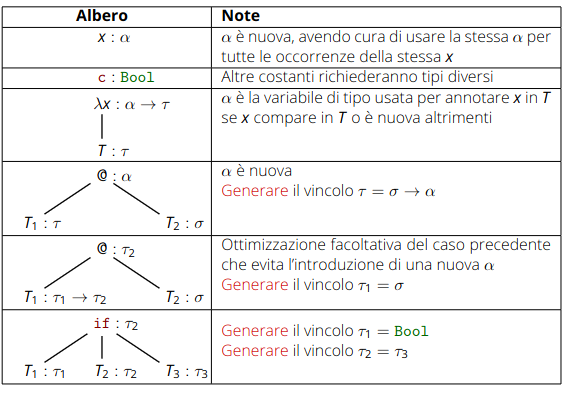
\includegraphics[scale = 0.7]{images/algoritmo di inferenza/Annotazione e vincoli.png}    
\end{center}

\ex{}{
\begin{multicols}{2}
[$\lambda x.x \:\:\text{\textcolor{red}{ True}}$]
    Albero annotato
    \begin{center}
    \begin{forest}
        [@ : \textcolor{red}{$\alpha$} [$\lambda x$ : \textcolor{red}{$\alpha \rightarrow \alpha$} [$x$ : \textcolor{red}{$\alpha$}]][True : \textcolor{green}{Bool}]]        
    \end{forest}
    \end{center}
    \pagebreak
    Vincoli generati

    $\alpha = \text{\textcolor{green}{Bool}}$
\end{multicols}
}

\ex{}{
\begin{multicols}{2}
[$\lambda f.\lambda x.f\:\:(f\:\:x)$]
    Albero annotato
    \begin{center}
    \begin{forest}
        [$\lambda f$ : \textcolor{red}{$\alpha \rightarrow \beta \rightarrow \delta$}[$\lambda x$ : \textcolor{red}{$\beta \rightarrow \delta$} [@ : \textcolor{red}{$\delta$}[$f$ : \textcolor{red}{$\alpha$}] [@ : \textcolor{red}{$\gamma$} [$f$ : \textcolor{red}{$\alpha$}] [$x$ : \textcolor{red}{$\beta$}]]]]]
    \end{forest}
    \end{center}
    \pagebreak
    Vincoli generati

    $\alpha = \beta \rightarrow \gamma$

    $\alpha = \gamma \rightarrow \delta$
\end{multicols}
}

\nt{Nell'ultimo esempio entrambe le $f$ hanno la stessa annotazione}

\subsection{Sistemi di equazioni e soluzioni}

\dfn{Sostituzione}{Una sostituzione $\theta$ è una funzione da variabili di tipo a espressioni di tipo. Scriviamo $\theta(\tau)$ per l'espressione ottenuta da $\tau$ sostituendo ogni $\alpha$ con $\theta (\alpha)$}

\dfn{Soluzione}{Dato un sistema di vincoli $\{\tau_i = \sigma_i\}_{1 \leq i \leq n}$ e una sostituzione $\theta$ diciamo che $\theta$ è soluzione (o unificatore) del sistema se $\theta(\tau_i) = \theta(\sigma_i)$ per ogni $1 \leq i \leq n$. Diciamo inoltre che $\theta$ è l’unificatore più generale del sistema
se ogni soluzione del sistema è ottenibile componendo $\theta$ con un’altra sostituzione}

\begin{center}
    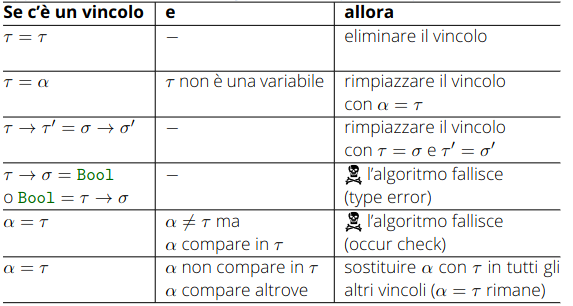
\includegraphics[scale = 0.7]{images/algoritmo di inferenza/Algoritmo di risoluzione.png}    
\end{center}

\nt{L'ordine in cui si applicano le trasformazioni non è importante. Se non si può applicare nessuna trasformazione l'algoritmo ha avuto successo}

\mprop{}{
\begin{itemize}
    \item In un numero finito di passi l'algoritmo ha successo o fallisce;
    \item Se l'algoritmo fallisce allora il sistema è insoddisfacibile;
    \item Se l'algoritmo ha successo:
    \begin{itemize}
        \item il sistema ha forma $\{\alpha_i = p_i\}_{1 \leq i \leq m}$ in cui ciascuna $\alpha_i$ compare una sola volta nel sistema;
        \item la sostituzione $\theta = \{\alpha_i \rightarrow p_i\}_{1 \leq i \leq m}$ è l'unificatore più generale del sistema iniziale, in particolare $\sigma(\tau_i) = \theta(\sigma_i))$ per ogni $\ \leq i \leq m$.
    \end{itemize}
\end{itemize}
}
\pagebreak
\ex{}{
\begin{center}
    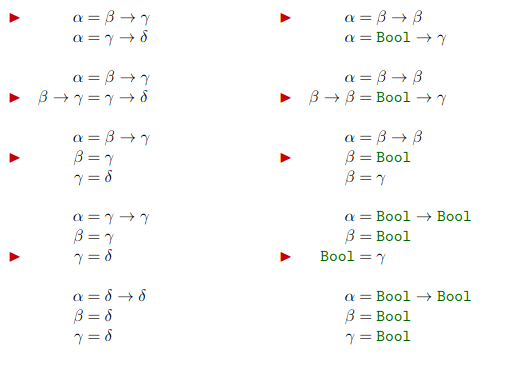
\includegraphics[scale = 0.7]{images/algoritmo di inferenza/Esempio.png}    
\end{center}
}


\ex{Esercizio}{
$(\lambda x.\lambda y. x\:\:y\:\:y) (\lambda a.a) b)$
\begin{multicols}{2}
\begin{center}

    \begin{forest}
    [@ : \textcolor{red}{n} [@ : \textcolor{red}{$\beta \rightarrow$ n}[$\lambda x$ : \textcolor{red}{$\alpha \rightarrow \beta \rightarrow $n }[$\lambda y$ : \textcolor{red}{$\beta \rightarrow$ n}[@ : \textcolor{red}{n}[@ : \textcolor{red}{$\epsilon$} [x : \textcolor{red}{$\alpha$}][y : \textcolor{red}{$\beta$}]][y : \textcolor{red}{$\beta$}]]]][$\lambda$ a : \textcolor{red}{$\gamma \rightarrow \gamma$}[a : \textcolor{red}{$\gamma$}]]] [b : \textcolor{red}{$\sigma$}]]
    \end{forest}
    
\end{center}
\pagebreak
$\alpha = \beta \rightarrow \epsilon$

$\epsilon = \beta \rightarrow$ n

$\alpha = \gamma \rightarrow \gamma$

$\beta = \sigma$
\end{multicols}
\pagebreak
Risoluzione:
\begin{multicols}{2}
$\begin{cases}
    \alpha = \beta \rightarrow \epsilon\\

    \epsilon = \beta \rightarrow \text{n}\\

    \alpha = \gamma \rightarrow \gamma\\

    \beta = \sigma
\end{cases}$

$\begin{cases}
    \alpha = \beta \rightarrow \epsilon\\

    \epsilon = \beta \rightarrow \text{n}\\

    \beta \rightarrow \epsilon = \gamma \rightarrow \gamma\\

    \beta = \sigma
\end{cases}$

$\begin{cases}
    \alpha = \beta \rightarrow \epsilon\\

    \epsilon = \beta \rightarrow \text{n}\\

    \beta = \gamma\\

    \epsilon = \gamma \\

    \beta = \sigma
\end{cases}$

$\begin{cases}
    \alpha = \gamma \rightarrow \epsilon\\

    \epsilon = \gamma \rightarrow \text{n}\\

    \beta = \gamma\\

    \epsilon = \gamma \\

    \gamma = \sigma
\end{cases}$

$\begin{cases}
    \alpha = \gamma \rightarrow \gamma \rightarrow \text{n}\\

    \epsilon = \gamma \rightarrow \text{n}\\

    \beta = \gamma\\

    \gamma \rightarrow \text{n} = \gamma \\

    \gamma = \sigma
\end{cases}$

$\begin{cases}
    \alpha = \gamma \rightarrow \gamma \rightarrow \text{n}\\

    \epsilon = \gamma \rightarrow \text{n}\\

    \beta = \gamma\\

     \gamma = \gamma \rightarrow \text{n}\\

    \gamma = \sigma
\end{cases}$

\textcolor{red}{\textbf{! OCCUR CHECK FAIL !}}

\end{multicols}

}

\section{Estensioni dell'algoritmo}

\dfn{Numeri interi}{Le costanti includono i numeri interi
$$c \in \{\text{False}, \text{True}, \:\:0, \:\:1,...\}$$

Le espressioni di tipo sono arricchite con il tipo \textcolor{green}{Int}
}

\nt{Se c'è un vincolo $\tau \rightarrow \sigma = \text{\textcolor{green}{Int}}$ o \textcolor{green}{Int} = \textcolor{green}{Bool} o \textcolor{green}{Bool} = \textcolor{green}{Int} l'algoritmo fallisce (\textcolor{red}{TYPE ERROR})}

\dfn{Liste}{Le costanti includono i costruttori canonici
$$c \in \{..., \:\:[\:],\:\:(:)\}$$

Ogni occorrenza di un costruttore fa uso di nuove variabili di tipo
}

\nt{
\begin{itemize}
    \item Se c'è un vincolo $[\tau] = [\sigma]$ rimpiazzarlo con $\tau = \sigma$;
    \item Se c'è un vincolo $[\tau] = \text{\textcolor{green}{Bool}}$ o $\text{\textcolor{green}{Bool}} = [\tau]$ o $[\tau] = \sigma_1 \rightarrow \sigma_2$ o ... l'algoritmo fallisce (\textcolor{red}{TYPE ERROR})
\end{itemize}
}

\dfn{Funzioni di libreria}{Le costanti includono le funzioni di libreria
$$c \in \{...,\:\:\text{id},\:\:\text{head},\:\:\text{tail},...\}$$

Ogni occorrenza di una funzione di libreria fa uso di nuove variabili di tipo
}

\dfn{Definizioni ricorsive}{
$$f = M$$
dove $f$ può comparire in $M$.
Il nome $f$ è trattato come ogni altra variabile. Alla fine dell'annotazione si genera il vincolo $\alpha = \tau$ dove $\alpha$ è la variabile di tipo associata a $f$ e $\tau$ è l'annotazione di $M$
}







\chapter{Dimostrazione di proprietà di funzioni}

\qs{}{Date una funzione e una specifica di ciò che la funzione dovrebbe calcolare, la funzione è corretta rispetto alla specifica?}

\qs{}{Date due funzioni (una corretta ma inefficiente e una efficiente ma più complessa da capire), sono equivalenti?}

\paragraph{Test:}

\begin{itemize}
    \item facile (soprattutto se il linguaggio non è imperativo);
    \item non è esaustivo (possono esserci casi non considerati).
\end{itemize}

\paragraph{Dimostrazione:}

\begin{itemize}
    \item difficile (soprattutto se il linguaggio è imperativo);
    \item è esaustiva.
\end{itemize}

\section{Dimostrazioni su numeri interi}

\begin{lstlisting}
foo :: Int -> Int -> Int -> Int
foo x y z | y < x       = foo y x z
          | z < y       = foo x z y
          | otherwise   = z
\end{lstlisting}

\qs{}{$\forall\:\: x,\:\:y,\:\:z = \text{max }\{x,\:\:y,\:\:z\}$ è una proprietà vera?}

Si possono fare dei test, ma saranno sempre in numero finito. Per cui è più conveniente cercare una dimostrazione.

\subsection{Dimostrazione per casi}

\nt{I numeri sono infinite, per cui non si può verificare il comportamento per ogni combinazione. Ma l'ordine tra i numeri è totale, per cui possiamo considerare un numero finito di casi che è esaustivo}

\begin{center}
    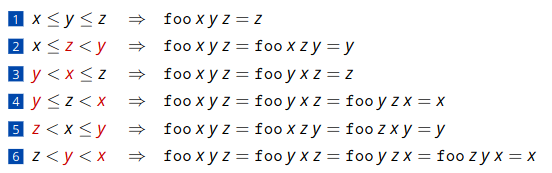
\includegraphics[scale = 0.7]{images/funzioni/Casi.png}    
\end{center}

\nt{Il codice è tutto ciò che serve per ragionare sui casi}

\subsection{Induzione}

\nt{L'approccio precedente è attuabile solo se il numero dei casi da prendere in considerazione è finito. Il principio di induzione permette di dimostrare una proprietà su un insieme infinito di casi}

\dfn{Il principio di induzione}{Data una proprietà $P(n)$ dei numeri naturali, se:
\begin{itemize}
    \item $P(0)$;
    \item $P(n)$ implica $P(n + 1)$ per ogni $n \in \bbN$.
\end{itemize}
allora $P(n)$ per ogni $n \in \bbN$
}
\begin{lstlisting}
exp :: Int -> Int -> Int -> Int
exp _ 0 = 1
exp x n = x * exp x (n - 1)
\end{lstlisting}
\ex{Esponenziale}{

Si vuole dimostrare che:
\begin{enumerate}
    \item $\forall\:\:x,\:\:m \geq 0,\:\:n\geq 0 : \text{exp } x\:\:(m + n) = \text{exp } x\:\:m * \text{exp} x |:\: n$;
    \item $\forall \:\:x, \:\:n : \text{exp }(x * x)\:\:n = \text{exp } x\:\:n * \text{exp } x\:\:n$.
\end{enumerate}
\pagebreak
\paragraph{Prima dimostrazione:}
\begin{center}
    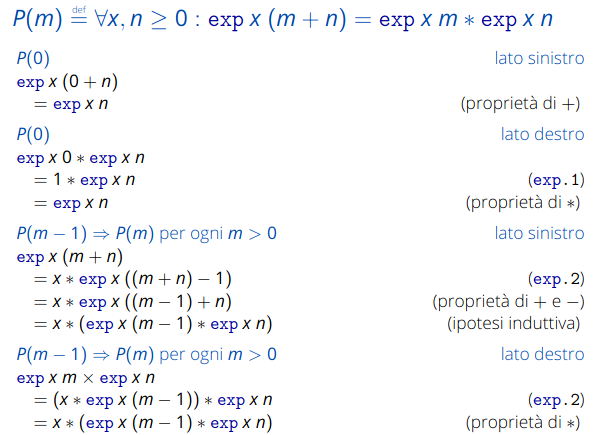
\includegraphics[scale = 0.7]{images/funzioni/Dim1.png}    
\end{center}
\paragraph{Seconda dimostrazione:}
\begin{center}
    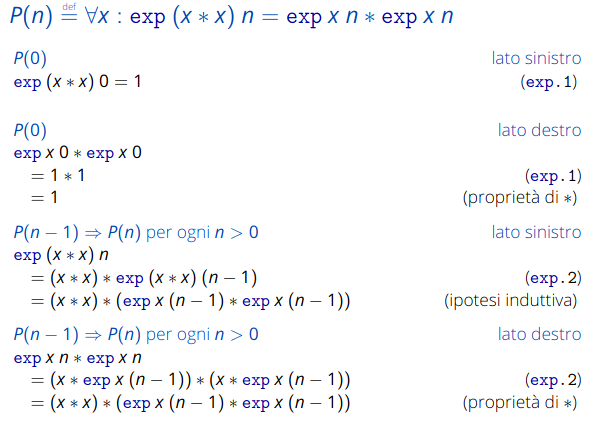
\includegraphics[scale = 0.7]{images/funzioni/Dim2.png}    
\end{center}
}

\dfn{Principio di induzione forte}{Data una proprietà $P(n)$ dei numeri naturali, se:
\begin{itemize}
    \item $(\forall \:\: m < n : P(m))\Rightarrow P(n)$, per ogni $n \in \bbN$.
\end{itemize}
allora $P(n)$ per ogni $n \in \bbN$
}

\nt{Il principio di induzione forte è equivalente al principio di induzione}

\section{Dimostrazioni sulle liste}

\dfn{Principio di induzione sulle liste finite}{
Data una proprietà $P(xs)$ delle liste, se:
\begin{itemize}
    \item $P([])$;
    \item $P(xs)$ implica $P(x\:\: :\:\:xs)$ per ogni $x$ e $xs$.
\end{itemize}
Allora $P(xs)$ per ogni lista finita $xs$.
}

\ex{Length}{
\begin{center}
    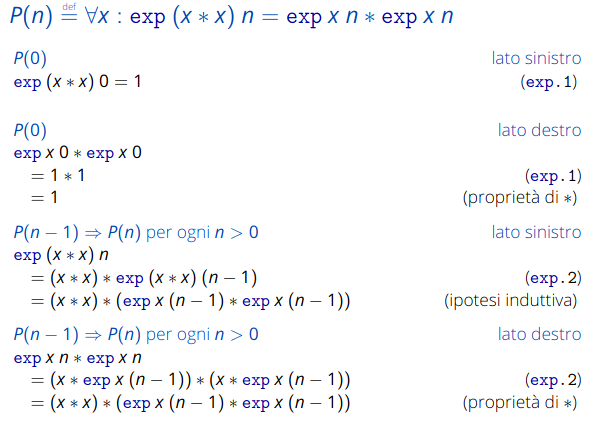
\includegraphics[scale = 0.7]{images/funzioni/Dim2.png}    
\end{center}
}
\nt{Può capitare, durante una dimostrazione, di osservare passaggi intuitivi di cui non si ha una prova. Per cui si possono assumere e poi dimostrare in seguito}

\section{Dimostrazioni sugli alberi}

\dfn{Principio di induzione sugli alberi}{
Data una proprietà $P(t)$, se:
\begin{itemize}
    \item $P(Leaf)$;
    \item $P(t_1) \wedge P(t_2)$ implica $P(Branch\:\:t_1 t_2)$ per ogni $x$, $t_1$ e $t_2$.
\end{itemize}
Allora  $P(t)$ per ogni albero (finito) $t$.
}

\ex{Trees}{
    \begin{center}
        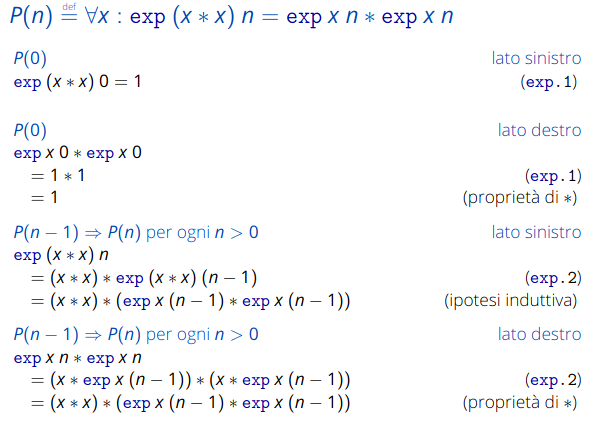
\includegraphics[scale = 0.7]{images/funzioni/Dim2.png}    
    \end{center}
}

\section{Dimostrazioni sulle funzioni di ordine superiore}

\dfn{Principio di estensionabilità}{
Due funzioni $f$ e $g$ sono uguali se producono lo stesso risultato
quando sono applicate allo stesso argomento. Formalmente:
$$(\forall x\: :\: f\: g = g\: x) \Leftrightarrow f = g$$
}

\nt{
È il principio che giustifica la regola di $\eta$-riduzione.    
}

\cor{proprietà della composizione funzionale}{
    \begin{center}
        \includegraphics[scale = 0.7]{images/funzioni/Proprietà.png}    
    \end{center}
}

\thm{Legge di fusione}{
Se:
\begin{itemize}
    \item $f\:a = b$;
    \item $f\:(g\:x\:y) = h\:x\:(f\:y)$;
\end{itemize}
allora
\begin{itemize}
    \item $f\:.\:\text{foldr}\:g\:a = \text{foldr}\:h\:b$.
\end{itemize}
}


\chapter{Java 8}

A un certo punto, nella storia di Java, si è deciso di effettuare un 
"\textit{restiling}" delle collection\footnote{Implementazioni delle
strutture dati più comuni, come liste, insiemi, mappe, etc.}. Per cui si
sono introdotti:
\begin{itemize}
    \item i metodi di default;
    \item lambda-espressioni: rendono il codice più compatto, modulare e
    leggibile.
\end{itemize}

\section{Lambda-espressioni}

\dfn{Lambda-espressione}{Una lambda-espressione è una funzione anonima
che può essere passata come parametro ad un metodo o ad un costruttore.
La sintassi è la seguente:
\begin{itemize}
    \item (parameters) $\rightarrow$ expression;
    \item (parameters) $\rightarrow$ \{ statements; \}.
\end{itemize}
}

\cor{Identità}{
L'Identità $\lambda x\: : \: \text{int}.x$ è:
\begin{itemize}
    \item $(x\: : \: \text{int}) \rightarrow x$;
    \item $(x\: : \: \text{int}) \rightarrow \{ \text{return}\: x; \}$.
\end{itemize}
}

\nt{In alcuni casi si può omettere il tipo dei parametri, in quanto
Java è in grado di inferirlo (raramente)}

\qs{}{Qual è il tipo dell'Identità?}

\dfn{Interfacce funzionali}{In Java 8 sono state introdotte le interfacce
funzionali, ovvero interfacce che hanno un solo metodo astratto. Esse
rappresentano il tipo delle lambda-espressioni. Per esempio, l'Identità
ha tipo Int che ritorna Int (quindi Int $\rightarrow$ Int, in Haskell)
}

\nt{Esistono interfacce funzionali già pronto, come per esempio
\textit{Predicate}, \textit{Consumer}, \textit{Function}, etc.}

\dfn{Method reference}{
Un method reference è un modo per riferirsi a un metodo. Aumenta la leggibilità
del codice.
La sintassi è la seguente: Type::methodName
}

\section{Compatibilità e metodi di default}

\dfn{Binary compatibility}{
Due versioni di una libreria sono binariamente compatibili se i file
binari continuano a funzionare anche con la nuova versione
}

\nt{
Se si modifica un software bisogna tener conto della backward compatibility,
ovvero la compatibilità con le versioni precedenti
}

\dfn{Source compatibility}{
Due versioni di una libreria sono sorgente compatibili se un programma esistente
continua a funzionare anche dopo essere stato ricompilato con la nuova versione
}

\dfn{Behavioural compatibility}{
Due versioni di una libreria sono behavioural compatibili se un programma
esistente continua a produrre lo stesso output con lo stesso input
}

\nt{Per mantenere la source compatibility tra Java 7 e Java 8, si è deciso
di introdurre i metodi di default}

\dfn{Metodi di default}{
I metodi di default sono metodi che possono essere implementati all'interno
di un'interfaccia. Essi permettono di aggiungere nuove funzionalità alle
interfacce senza rompere la compatibilità con le versioni precedenti. Per
fare ciò vengono aggiunti metodi opzionali (che possono essere implementati o meno).
Se non vengono implementati, viene usata l'implementazione di default
}

\nt{
I metodi di default vengono usati per modificare molte interfacce di Java collections
per rendere più semplice l'uso delle lambda-espressioni e mantenere la backward compatibility
}

\section{L'interfaccia Function}

\dfn{Function$\langle$T, R$\rangle$}{
L'interfaccia Function$\langle$T, R$\rangle$ è un'interfaccia funzionale
che rappresenta una funzione che prende un parametro di tipo T e ritorna
un parametro di tipo R. Essa ha un solo metodo astratto:
\begin{itemize}
    \item R apply(T t).
\end{itemize}
Oltre a questo presenta il metodo di default:
\begin{itemize}
    \item Function$\langle$T, R$\rangle$ andThen(Function$\langle$? super R, ? extends V$\rangle$ after) che 
    ritorna una funzione che prima applica la funzione corrente e poi la funzione after.
\end{itemize}   
}

\end{document}